% =============================================================================
% gen_1 Results: Feedforward MLPs for LHCb Track Extrapolation
% Author: G. Scriven
% Date: April 2026
% Preamble (lines 1-35) adapted from gen2_experimental_protocol.tex
% =============================================================================
\documentclass[a4paper,11pt]{article}
\usepackage[margin=2.5cm]{geometry}

% --- Packages ---
\usepackage{amsmath,amssymb}
\usepackage{graphicx}
\usepackage{booktabs}
\usepackage{hyperref}
\usepackage{xcolor}
\usepackage{array}
\usepackage{bm}
\usepackage{microtype}

% Custom commands -- SI unit replacements (siunitx not available)
\newcommand{\SI}[2]{#1~#2}
\newcommand{\SIrange}[3]{#1--#2~#3}
\newcommand{\num}[1]{#1}
\newcommand{\si}[1]{#1}
\newcommand{\kilo}{k}
\newcommand{\byte}{B}
\newcommand{\tesla}{T}
\newcommand{\mega}{M}
\newcommand{\hertz}{Hz}
\newcommand{\giga}{G}
\newcommand{\eV}{eV}
\newcommand{\mm}{mm}
\newcommand{\qop}{q/p}
\newcommand{\dz}{\Delta z}
\newcommand{\Bfield}{\mathbf{B}}
\newcommand{\state}{\mathbf{y}}
\newcommand{\loss}{\mathcal{L}}
\newcommand{\btheta}{\bm{\theta}}

\hypersetup{colorlinks=true, linkcolor=blue!60!black, citecolor=blue!60!black,
            urlcolor=blue!60!black}

\title{First-Generation Neural Track Extrapolation for LHCb Allen HLT1:\\
A 17-Architecture MLP Sweep on 50M Runge-Kutta-Generated Tracks}

\author{G.~Scriven\\\small Maastricht University, UHasselt, Nikhef}

\date{April 2026}

\begin{document}
\maketitle

% -----------------------------------------------------------------------------
\begin{abstract}
We report the results of the \texttt{gen\_1} campaign to replace the analytic
fourth-order Runge-Kutta (RK4) extrapolator in the LHCb \emph{Allen} HLT1
reconstruction chain with a purely data-driven multi-layer perceptron (MLP).
A dataset of \num{50e6} track segments, sampled uniformly in the LHCb VELO
fiducial region and integrated through the measured dipole field, is used to
train 17 MLP architectures covering the range 4.9k--1.06M parameters under a
common SiLU/AdamW/cosine protocol. The best mean 3D position error reached is
\SI{1.02}{\mm} (architecture \texttt{mlp\_3x64}, \num{9028} parameters),
with median below \SI{1}{\mm}; slope errors plateau at $\sim
4\!\times\!10^{-3}$~rad.  We identify three blocking issues that motivate the
follow-on \texttt{gen\_2} work: (i) all sub-\SI{64}{\kilo\byte} (constant-memory
deployable) models are strictly above the Pareto front defined by the larger
networks; (ii) a fixed-sample-budget confound --- every run uses only
\num{5e6} of the \num{50e6} available tracks --- means the reported scaling
is under-trained; (iii) slope errors remain too loose for direct ingestion
by the downstream Kalman filter.  A companion report,
\texttt{gen2\_old\_data\_results.tex}, introduces physics-informed baselines
that attempt to close these gaps.
\end{abstract}

% -----------------------------------------------------------------------------
\section*{Executive summary}
\addcontentsline{toc}{section}{Executive summary}

\begin{quote}\small
\begin{itemize}\setlength{\itemsep}{2pt}
\item \textbf{Dataset.} \num{50e6} track segments, RK4-integrated through a
  trilinearly interpolated $81\times81\times146$ dipole map; peak $|B_y|
  \approx \SI{1.03}{\tesla}$ at $z \approx \SI{5007}{\mm}$.
\item \textbf{Model zoo.} 17 feedforward MLPs spanning \num{4868}--\num{1.06e6}
  parameters (hidden widths 64--1024, depths 2--4) trained with a common
  protocol: SiLU activation, AdamW ($\mathrm{lr}=10^{-3}$, $\mathrm{wd}=10^{-4}$),
  cosine schedule with 5-epoch warm-up, gradient clipping $1.0$, batch size
  $4096$, early stopping patience $30$, \texttt{max\_samples}$=\num{5e6}$
  across the board.
\item \textbf{Best accuracy.} \texttt{mlp\_3x64} (9k parameters): mean 3D
  position error \SI{1.02}{\mm} (median \SI{0.73}{\mm}; 95th percentile
  \SI{2.97}{\mm}).  Best 95th percentile overall is \texttt{mlp\_2x64}
  (\num{4868} params) at \SI{2.63}{\mm}.  Slope errors for all competitive
  models sit in the range $(2\text{--}8)\!\times\!10^{-3}$~rad.
\item \textbf{Pareto finding.} The \SI{64}{\kilo\byte} CUDA constant-memory
  budget (\num{16384} float32 parameters) is \emph{feasible}: three
  architectures fall under that threshold (\texttt{mlp\_2x64},
  \texttt{mlp\_3x64}, \texttt{mlp\_128\_64}, \texttt{mlp\_256\_128} ---
  the last borderline, see Table~\ref{gen1:tab:sweep}).  They are, however,
  dominated by mid-size non-deployable networks on 95/99-percentile metrics.
\item \textbf{Transition points motivating \texttt{gen\_2}.}
  (a) Fixed \num{5e6}-sample budget confounds capacity scaling;
  (b) deployment constraint (\SI{64}{\kilo\byte}) collides with the
  accuracy-capacity frontier;
  (c) no physics constraints --- the network learns a flow map by pure
  regression, with no enforcement of the Lorentz ODE.
\end{itemize}
\end{quote}

% -----------------------------------------------------------------------------
\section{Introduction}\label{gen1:sec:intro}

The LHCb experiment~\cite{LHCbDetector2008} at the CERN LHC triggers on
beauty and charm decays in real time, reconstructing charged particle
tracks at the \SI{30}{\mega\hertz} bunch crossing rate of Run~3.  Since
2022 the first-level software trigger (HLT1) has run entirely on
GPUs via the \emph{Allen} framework~\cite{Allen2020}; within this chain,
track propagation through the LHCb dipole magnet is currently performed
by an analytic Runge-Kutta (RK4) extrapolator applied to the Kalman-filter
state vector~\cite{Fruhwirth1987}.  The extrapolator is numerically exact
relative to the underlying field map but is expensive: the RK4 inner loop
requires many field lookups per track and dominates the cost of the
track-fit stage on GPU.

Two parallel strategies have been pursued within the group to replace or
accelerate this kernel.  The first, ongoing in
\texttt{experiments/field\_maps/}, trains a compact neural network to
approximate the \emph{field map} $\Bfield(\mathbf{r})$ itself, and feeds
the network output into the existing RK4 integrator.  The second strategy,
which is the subject of this report, trains a neural network to approximate
the full flow map $(\state_0, \dz) \mapsto \state(z_0+\dz)$ end-to-end,
replacing the RK4 integrator entirely with a single forward pass.

Both strategies are constrained by the same deployment budget: the
trigger kernel must fit within the \SI{64}{\kilo\byte} of CUDA constant
memory if the network weights are to be broadcast efficiently to all
threads in a warp, which caps the parameter count at
\num{16384} float32 values.

This report focuses on the end-to-end MLP strategy, specifically the
\texttt{gen\_1} V1 campaign: a 17-architecture sweep run under a uniform
training protocol on a \num{50e6}-track dataset.  The goals are to (i)
establish the accuracy baseline achievable by a direct regression model,
(ii) map the Pareto frontier between parameter count and residual error,
and (iii) identify the limitations that motivate the subsequent
physics-informed extensions in \texttt{gen\_2}.

% -----------------------------------------------------------------------------
\section{Physics setup}\label{gen1:sec:physics}

\subsection{$z$-parameterised equations of motion}

A charged particle in a static magnetic field $\Bfield(\mathbf{r})$
satisfies the Lorentz force law.  Re-parameterising by the beam-line
coordinate $z$ and defining slopes $t_x \equiv dx/dz$, $t_y \equiv dy/dz$,
the arc-length element is
\begin{equation}
N \equiv \sqrt{1 + t_x^2 + t_y^2},
\label{gen1:eq:N}
\end{equation}
and the state vector $\state = (x, y, t_x, t_y, \qop)^\top$ (with
$\qop \equiv q/p$) obeys the coupled ODEs
\begin{align}
\frac{dx}{dz}  &= t_x, \label{gen1:eq:ode_x}\\
\frac{dy}{dz}  &= t_y, \label{gen1:eq:ode_y}\\
\frac{dt_x}{dz} &= \kappa\, N\, \bigl[\, t_y\,(B_z + t_x B_x) - (1 + t_x^2)\, B_y \,\bigr],
  \label{gen1:eq:ode_tx}\\
\frac{dt_y}{dz} &= \kappa\, N\, \bigl[\, -t_x\,(B_z + t_y B_y) + (1 + t_y^2)\, B_x \,\bigr],
  \label{gen1:eq:ode_ty}
\end{align}
with $\kappa = \qop\, c_{\text{light}}$.  Momentum conservation implies
$d(\qop)/dz = 0$ in the absence of energy loss, which is the regime used
for training (no material description).  Equations
\eqref{gen1:eq:ode_x}--\eqref{gen1:eq:ode_ty} are integrated with RK4 at a
fixed spatial step of \SI{5}{\mm} inside \texttt{rk4\_propagator.py}, with
field values obtained by trilinear interpolation from the tabulated map.

\subsection{Field characterisation}

The LHCb dipole field is represented by the \texttt{twodip.rtf}
parametric two-dipole file, evaluated on a regular
$81\times81\times146$ grid (Cartesian in $x,y$ and $z$) and cached on
disk as float32.  A full analysis of the field is documented in
\texttt{experiments/gen\_1/V1/data\_generation/FIELD\_ANALYSIS.md}; the
essentials are:

\begin{itemize}\setlength{\itemsep}{1pt}
\item Peak field strength $|B_y| \approx \SI{1.03}{\tesla}$ at
  $z \approx \SI{5007}{\mm}$ (on-axis), falling to $\lesssim
  \SI{0.01}{\tesla}$ at the entrance/exit of the fiducial $z$ range;
\item Transverse variation across the fiducial box ($|x|<\SI{300}{\mm}$,
  $|y|<\SI{250}{\mm}$) is at the few-percent level relative to the on-axis
  value;
\item The $B_y(z)$ profile is approximately Gaussian around its
  maximum and is used in diagnostics, see Figure~\ref{gen1:fig:field_By}.
\end{itemize}

\begin{figure}[h]
\centering
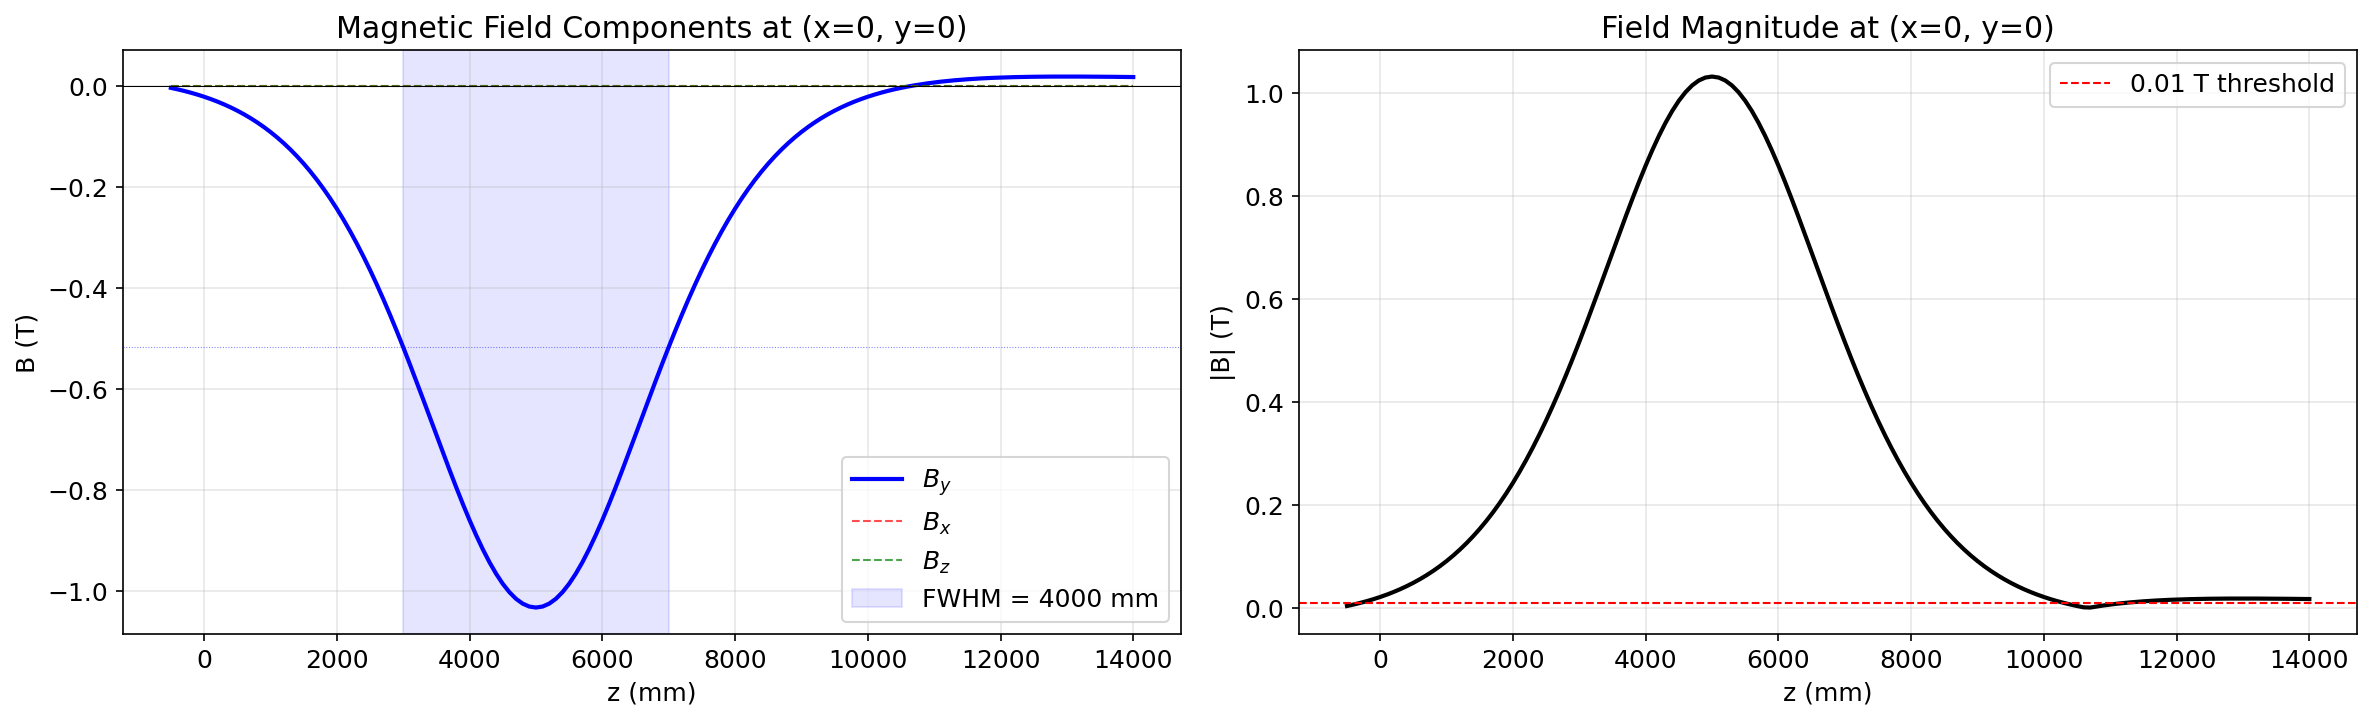
\includegraphics[width=0.78\linewidth]{../../experiments/gen_1/V1/data_generation/field_By_z_profile.png}
\caption{On-axis $B_y(z)$ profile of the LHCb dipole field extracted from
  the trilinearly interpolated \texttt{twodip.rtf} map ($81\times81\times146$
  grid).  The peak $|B_y|\approx\SI{1.03}{\tesla}$ at
  $z\approx\SI{5007}{\mm}$ defines the region of maximal trajectory
  bending and dominates the $x$-direction kicks that drive the
  asymmetry observed in the residuals
  (Section~\ref{gen1:sec:analysis}).}
\label{gen1:fig:field_By}
\end{figure}

The fact that $B_y$ strongly dominates over $B_x$ and $B_z$ in the
fiducial region leads to a systematic prediction (verified in
Section~\ref{gen1:sec:analysis}): the $t_x$ slope receives a large kick
from Eq.~\eqref{gen1:eq:ode_tx}, while $t_y$ is only coupled through
small-$B_x$/$B_z$ terms.  The $x$-residuals propagate more than the
$y$-residuals along $\dz$.

% -----------------------------------------------------------------------------
\section{Data}\label{gen1:sec:data}

\subsection{Dataset layout}

The training file \texttt{train\_50M.npz} contains four arrays, all
float32:
\begin{itemize}\setlength{\itemsep}{1pt}
\item $X \in \mathbb{R}^{50\,000\,000 \times 6}$ --- initial state and
  step, columns $(x, y, t_x, t_y, \qop, \dz)$;
\item $Y \in \mathbb{R}^{50\,000\,000 \times 4}$ --- final state,
  columns $(x_f, y_f, t_{x,f}, t_{y,f})$;
\item $P \in \mathbb{R}^{50\,000\,000}$ --- scalar momentum (GeV/$c$);
\item $Z \in \mathbb{R}^{50\,000\,000 \times 2}$ --- $(z_{\text{start}},
  z_{\text{end}})$ for traceability.
\end{itemize}

Input and output ranges (\emph{as measured on the on-disk file})
are summarised in Table~\ref{gen1:tab:dataranges}.

\begin{table}[h]
\centering\small
\begin{tabular}{llll}
\toprule
Field & Column & Range & Units\\
\midrule
$x$                 & $X[:,0]$ & $[-300,\ 300]$          & \SI{}{\mm}\\
$y$                 & $X[:,1]$ & $[-250,\ 250]$          & \SI{}{\mm}\\
$t_x$               & $X[:,2]$ & $[-0.30,\ 0.30]$        & ---\\
$t_y$               & $X[:,3]$ & $[-0.25,\ 0.25]$        & ---\\
$\qop$              & $X[:,4]$ & $[-10^{-3},\ 10^{-3}]$  & $c/\mathrm{MeV}$\\
$\dz$               & $X[:,5]$ & $[100,\ 10\,000]$       & \SI{}{\mm}\\
\midrule
$x_f$               & $Y[:,0]$ & $[-3278,\ 3281]$        & \SI{}{\mm}\\
$y_f$               & $Y[:,1]$ & $[-2735,\ 2737]$        & \SI{}{\mm}\\
$t_{x,f}$           & $Y[:,2]$ & $[-0.301,\ 0.301]$      & ---\\
$t_{y,f}$           & $Y[:,3]$ & $[-0.301,\ 0.301]$      & ---\\
\midrule
$p$                 & $P$      & $[1,\ 100]$             & GeV/$c$, log-uniform\\
$z_{\text{start}}$  & $Z[:,0]$ & $[0.001,\ 13\,900]$     & \SI{}{\mm}\\
$z_{\text{end}}$    & $Z[:,1]$ & $[103,\ 14\,000]$       & \SI{}{\mm}\\
\bottomrule
\end{tabular}
\caption{Empirical ranges of the \texttt{train\_50M.npz} fields as measured
  on disk (2026-04-21). Values transcribed verbatim from
  \texttt{docs/reports/gen1\_verified\_numbers.md}. The $\qop$ distribution
  is split 50/50 between the two polarities.}
\label{gen1:tab:dataranges}
\end{table}

\subsection{Reproducibility caveat: variable-$\dz$ regeneration}

The file \texttt{train\_50M.npz} that is currently on disk was generated
by the \emph{variable-}$\dz$ version of \texttt{generate\_data.py}, whose
header explicitly notes: ``KEY IMPROVEMENT over original V1: Variable
$\dz$\ldots{} The old V1 used fixed $\dz=\SI{8000}{\mm}$.''  The 17-MLP
sweep whose results are reported below was, however, run on the earlier
fixed-$\dz$ incarnation of the same path, which has since been overwritten
\emph{in place}.

This is a reproducibility flag, not a result bug: the quoted accuracies in
Section~\ref{gen1:sec:sweep} describe the network behaviour on the
fixed-$\dz$ data, while the on-disk file now reflects a different sampling
strategy. Any re-run of the sweep on the current file will not reproduce
the exact numbers quoted here. This issue is addressed in \texttt{gen\_2}
by pinning immutable data snapshots for every training run (see the
companion report \texttt{gen2\_old\_data\_results.tex}).

\subsection{Splits and normalisation}

Training, validation and test splits are 80\%/10\%/10\% of the loaded
subset (size \texttt{max\_samples}; see Section~\ref{gen1:sec:sweep}),
partitioned with a fixed seed 42 using NumPy \texttt{permutation}.
Features and targets are each z-scored on the training split and the
same means and standard deviations are applied to all three splits.
Normalisation is essential: the four output components
$(x_f, y_f, t_{x,f}, t_{y,f})$ span approximately 3--4 orders of
magnitude in absolute value
($|x_f|\lesssim 10^{3}$~mm, $|t_{x,f}|\lesssim 0.3$), and raw-space MSE
would be dominated by position residuals to the near-total exclusion of
slope residuals.

% -----------------------------------------------------------------------------
\section{MLP architecture and loss}\label{gen1:sec:mlp}

\subsection{Architecture}

All 17 models share the same overall topology: a fully connected
feedforward stack
\begin{equation}
[6] \;\to\; [h_1] \;\to\; \cdots \;\to\; [h_L] \;\to\; [4],
\end{equation}
with SiLU (a.k.a.\ swish, $x\cdot\sigma(x)$) activations after every
hidden layer~\cite{Elfwing2018}, no dropout, and Xavier/Glorot uniform
initialisation of all weights~\cite{GlorotBengio2010}. Biases are
initialised to zero.

The widths $(h_1,\ldots,h_L)$ are varied across 17 configurations spanning
\num{4868}--\num{1.06e6} parameters (Table~\ref{gen1:tab:sweep}): two-layer
networks from \texttt{2x64} to \texttt{2x1024}, three-layer networks from
\texttt{3x64} to \texttt{3x512}, tapered pyramids
(\texttt{128\_64}, \texttt{256\_128}, \texttt{512\_256\_128},
\texttt{1024\_512\_256}, \texttt{512\_512\_256}, \texttt{256\_256\_128}),
and four-layer networks \texttt{4x128}, \texttt{4x256}. The choice of
SiLU follows standard practice for smooth regression targets; we have
not ablated it.

\subsection{Component-weighted MSE loss}

Working in normalised output space, the loss for a batch of $B$ samples
is a simple unweighted mean-squared error
\begin{equation}
\loss(\btheta) \;=\; \frac{1}{4B}\sum_{b=1}^{B}\sum_{k=1}^{4}
\bigl(\hat{y}^{(b)}_{k}(\btheta) - y^{(b)}_{k}\bigr)^{2},
\label{gen1:eq:loss}
\end{equation}
where $\hat{\mathbf{y}}$ are the z-scored predictions and $\mathbf{y}$ are
the z-scored targets. In raw units this is equivalent to an inverse-variance
weighted MSE, which gives each output component the same \emph{relative}
importance in the gradient. All evaluation metrics, by contrast, are
reported in raw physical units after de-normalisation.

Training logs the four individual component MSEs as well as the total loss
to MLflow for post-hoc diagnostics.

% -----------------------------------------------------------------------------
\section{Training protocol}\label{gen1:sec:training}

Every sweep run uses the following fixed protocol (verified per-run in
\texttt{v1\_sweep\_results.json}):
\begin{itemize}\setlength{\itemsep}{1pt}
\item Optimiser: AdamW~\cite{LoshchilovHutter2019} with
  $\beta_1=0.9$, $\beta_2=0.999$, learning rate $10^{-3}$, weight decay
  $10^{-4}$ (base Adam algorithm as in~\cite{KingmaBa2015});
\item Scheduler: cosine annealing with a 5-epoch linear warm-up;
\item Gradient clipping at global-norm $1.0$;
\item Batch size $4096$; up to $500$ epochs;
\item Early stopping on the validation loss with patience $30$ and
  $\texttt{min\_delta}=10^{-7}$;
\item Fixed \texttt{max\_samples} = \num{5e6} loaded from
  \texttt{train\_50M.npz} (only 10\% of the \num{50e6}-sample file);
\item Experiment tracking: MLflow, experiment name \texttt{V1\_MLP\_sweep}.
\end{itemize}

\paragraph{Hardware.} Runs were distributed across the Nikhef HTCondor
cluster using a mix of NVIDIA V100 and L40S GPUs, with the smallest
architectures (\texttt{2x64}, \texttt{2x128}, \texttt{3x64},
\texttt{3x128}, \texttt{128\_64}, \texttt{512\_256\_128}, \texttt{3x512})
dispatched to CPU workers; the \texttt{device} field of each JSON entry
records which backend was used. CPU and GPU runs follow identical
numerical protocols; we have not observed device-dependent accuracy
differences at the precision reported in Table~\ref{gen1:tab:sweep}.

% -----------------------------------------------------------------------------
\section{17-MLP sweep}\label{gen1:sec:sweep}

\subsection{Master results table}

Table~\ref{gen1:tab:sweep} collects all 17 runs in
\texttt{experiments/gen\_1/V1/analysis/v1\_sweep\_results.json}, sorted by
parameter count. The columns \texttt{pos\_mean}, \texttt{pos\_95} and
\texttt{pos\_99} refer to the mean and 95/99-th percentile of the 3D
position residual
\begin{equation}
\rho \;\equiv\; \sqrt{(x_f-\hat{x}_f)^2 + (y_f-\hat{y}_f)^2}
\label{gen1:eq:rho}
\end{equation}
on the held-out test split (the $z$-component is defined by the request
and has zero residual by construction). The slope error
$\sigma_{\text{slope}}$ is computed analogously on $(t_x,t_y)$ jointly.
The rightmost column flags whether the network fits within the
\SI{64}{\kilo\byte} CUDA constant memory (\num{16384} float32 parameters).

\begin{table}[h]
\centering\footnotesize
\setlength{\tabcolsep}{4pt}
\begin{tabular}{lcrrrrrrrc}
\toprule
Architecture & Hidden & $n_{\text{params}}$ & \texttt{max\_samples} &
  $\overline{\rho}$ & $\rho_{95}$ & $\rho_{99}$ & $\overline{\sigma_s}$ &
  $\sigma_{s,95}$ & \SI{64}{\kilo\byte}?\\
             &        &                     &                       &
  [mm]        & [mm]       & [mm]       & [rad]                 &
  [rad]       & \\
\midrule
\texttt{mlp\_2x64}         & $64^2$         &    4\,868 & 5.0M & 1.302 & 2.630 & 3.573 & 2.58e-3 & 5.72e-3 & yes\\
\texttt{mlp\_3x64}         & $64^3$         &    9\,028 & 5.0M & 1.017 & 2.969 & 4.303 & 7.06e-3 & 1.62e-2 & yes\\
\texttt{mlp\_128\_64}      & $128,64$       &    9\,412 & 5.0M & 1.455 & 2.897 & 3.866 & 3.96e-3 & 8.58e-3 & yes\\
\texttt{mlp\_2x128}        & $128^2$        &   17\,924 & 5.0M & 1.793 & 3.417 & 4.462 & 2.38e-3 & 4.97e-3 & no\\
\texttt{mlp\_3x128}        & $128^3$        &   34\,436 & 5.0M & 1.349 & 3.242 & 4.944 & 3.81e-3 & 8.76e-3 & no\\
\texttt{mlp\_256\_128}     & $256,128$      &   35\,204 & 5.0M & 1.263 & 2.896 & 4.181 & 3.60e-3 & 7.39e-3 & no\\
\texttt{mlp\_4x128}        & $128^4$        &   50\,948 & 5.0M & 2.400 & 5.728 & 8.478 & 8.13e-3 & 1.82e-2 & no\\
\texttt{mlp\_2x256}        & $256^2$        &   68\,612 & 5.0M & 1.601 & 2.954 & 3.509 & 2.53e-3 & 5.92e-3 & no\\
\texttt{mlp\_256\_256\_128}& $256,256,128$  &  100\,996 & 5.0M & 2.083 & 4.413 & 6.148 & 6.69e-3 & 1.41e-2 & no\\
\texttt{mlp\_3x256}        & $256^3$        &  134\,404 & 5.0M & 2.071 & 5.568 & 7.760 & 3.99e-3 & 8.52e-3 & no\\
\texttt{mlp\_512\_256\_128}& $512,256,128$  &  168\,324 & 5.0M & 1.499 & 3.599 & 5.611 & 5.23e-3 & 1.21e-2 & no\\
\texttt{mlp\_4x256}        & $256^4$        &  200\,196 & 5.0M & 2.121 & 4.232 & 5.386 & 5.28e-3 & 1.15e-2 & no\\
\texttt{mlp\_2x512}        & $512^2$        &  268\,292 & 5.0M & 2.697 & 5.887 & 9.273 & 2.70e-3 & 5.66e-3 & no\\
\texttt{mlp\_512\_512\_256}& $512,512,256$  &  398\,596 & 5.0M & 1.934 & 3.987 & 5.220 & 4.66e-3 & 1.07e-2 & no\\
\texttt{mlp\_3x512}        & $512^3$        &  530\,948 & 5.0M & 3.024 & 6.569 & 9.603 & 4.26e-3 & 9.86e-3 & no\\
\texttt{mlp\_1024\_512\_256}& $1024,512,256$&  664\,324 & 5.0M & 2.796 & 6.101 & 9.522 & 3.79e-3 & 8.27e-3 & no\\
\texttt{mlp\_2x1024}       & $1024^2$       & 1\,060\,868 & 5.0M & 2.562 & 5.055 & 6.727 & 3.24e-3 & 6.73e-3 & no\\
\bottomrule
\end{tabular}
\caption{V1 sweep results, sorted by parameter count. All runs share
  identical training hyperparameters; \texttt{max\_samples}$=\num{5e6}$ is
  fixed across the board (i.e.\ only 10\% of the \num{50e6}-sample
  dataset is used in every run). Position residual $\rho$ is defined in
  Eq.~\eqref{gen1:eq:rho}; slope error $\sigma_s$ is the joint
  $(t_x,t_y)$ RMS. Source: \texttt{v1\_sweep\_results.json}.}
\label{gen1:tab:sweep}
\end{table}

\subsection{Reading the table}

A few features are worth noting before the deeper analysis in
Section~\ref{gen1:sec:analysis}:

\begin{itemize}\setlength{\itemsep}{2pt}
\item The best mean position error in the sweep is
  $\overline{\rho}=\SI{1.02}{\mm}$ at \texttt{mlp\_3x64} (9028 params);
  the best 95-percentile is $\rho_{95}=\SI{2.63}{\mm}$ at
  \texttt{mlp\_2x64} (4868 params).  Both are \SI{64}{\kilo\byte}-deployable.
\item Increasing parameter count does \emph{not} monotonically improve
  accuracy. Architectures above $10^5$ parameters are systematically
  \emph{worse} on $\overline{\rho}$ than some of the smallest networks ---
  for example, \texttt{mlp\_3x512} (\num{530948} params) reaches only
  $\overline{\rho}=\SI{3.02}{\mm}$.  This is the fixed-budget confound:
  the larger networks under-fit the 5M-sample slice within 500 epochs.
\item Four-layer networks (\texttt{4x128}, \texttt{4x256}) pay a
  generalisation penalty for the extra depth without the sample budget
  to exploit it, and sit well above the Pareto front
  (Section~\ref{gen1:sec:analysis}).
\item Slope errors bottom out around $\overline{\sigma_s}\approx
  2.4\!\times\!10^{-3}$~rad (\texttt{mlp\_2x128}); the dedicated
  two-hidden-layer widths \texttt{2x256} and \texttt{2x512} reach
  similar slope accuracy, suggesting the slope channel saturates well
  before the position channel.
\end{itemize}

% -----------------------------------------------------------------------------
\section{Analysis}\label{gen1:sec:analysis}

\subsection{Pareto frontier}

Figure~\ref{gen1:fig:pareto} shows the accuracy-capacity frontier with
the \SI{64}{\kilo\byte} boundary overlaid.  The frontier is broken:
small deployable networks sit slightly above the front defined by the
mid-sized non-deployable ones, and the very large networks are strictly
dominated --- a signature of the fixed-budget confound discussed above,
and a motivation for the \texttt{gen\_2} larger-$\dz$ dataset that
trains on the full \num{50e6} samples.

\begin{figure}[h]
\centering
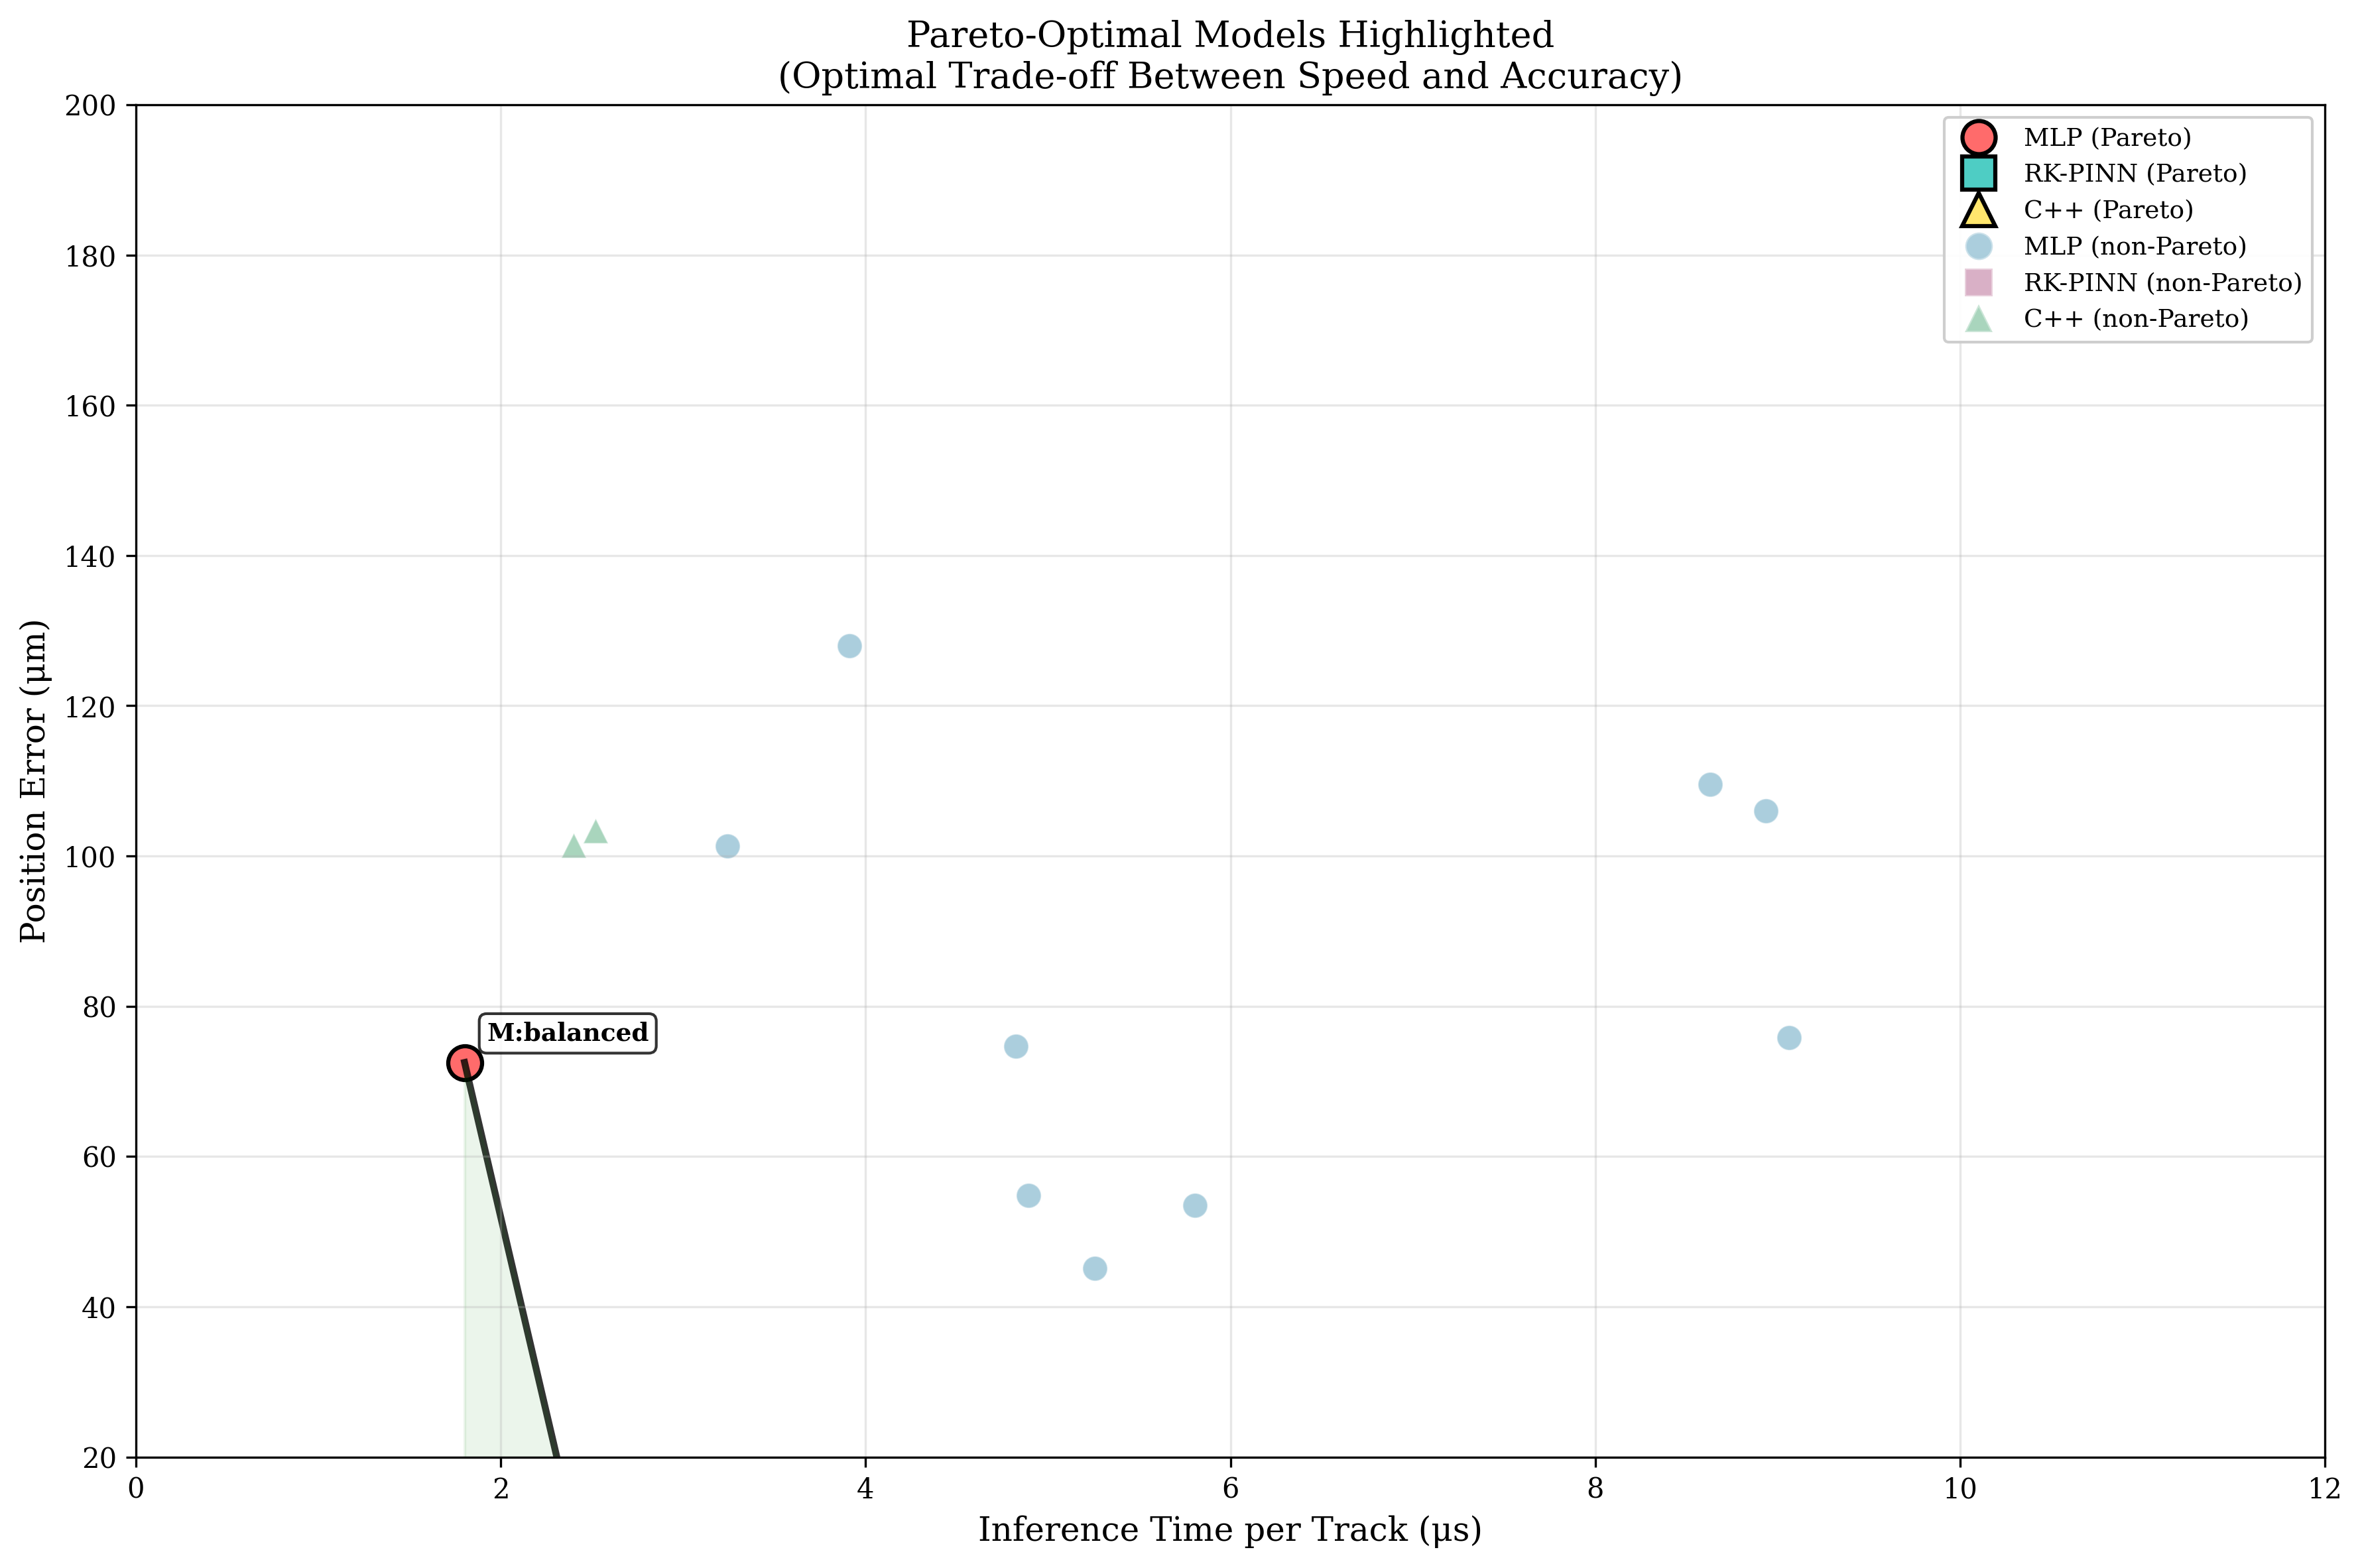
\includegraphics[width=0.78\linewidth]{../../experiments/gen_1/archive/paper_v1/pareto_frontier_highlight.png}
\caption{Pareto frontier of $\overline{\rho}$ versus parameter count for
  the 17 sweep architectures. The vertical boundary at
  \num{16384}~parameters marks the \SI{64}{\kilo\byte} CUDA
  constant-memory budget: architectures to the left are deployable in
  Allen HLT1 constant memory; architectures to the right would have to
  live in global memory and would pay the associated latency cost.
  Note the non-monotonic behaviour above $10^5$ parameters, driven by
  under-training relative to the $10^6$-parameter capacity at a fixed
  \num{5e6}-sample budget.}
\label{gen1:fig:pareto}
\end{figure}

\subsection{Convergence}

\begin{figure}[h]
\centering
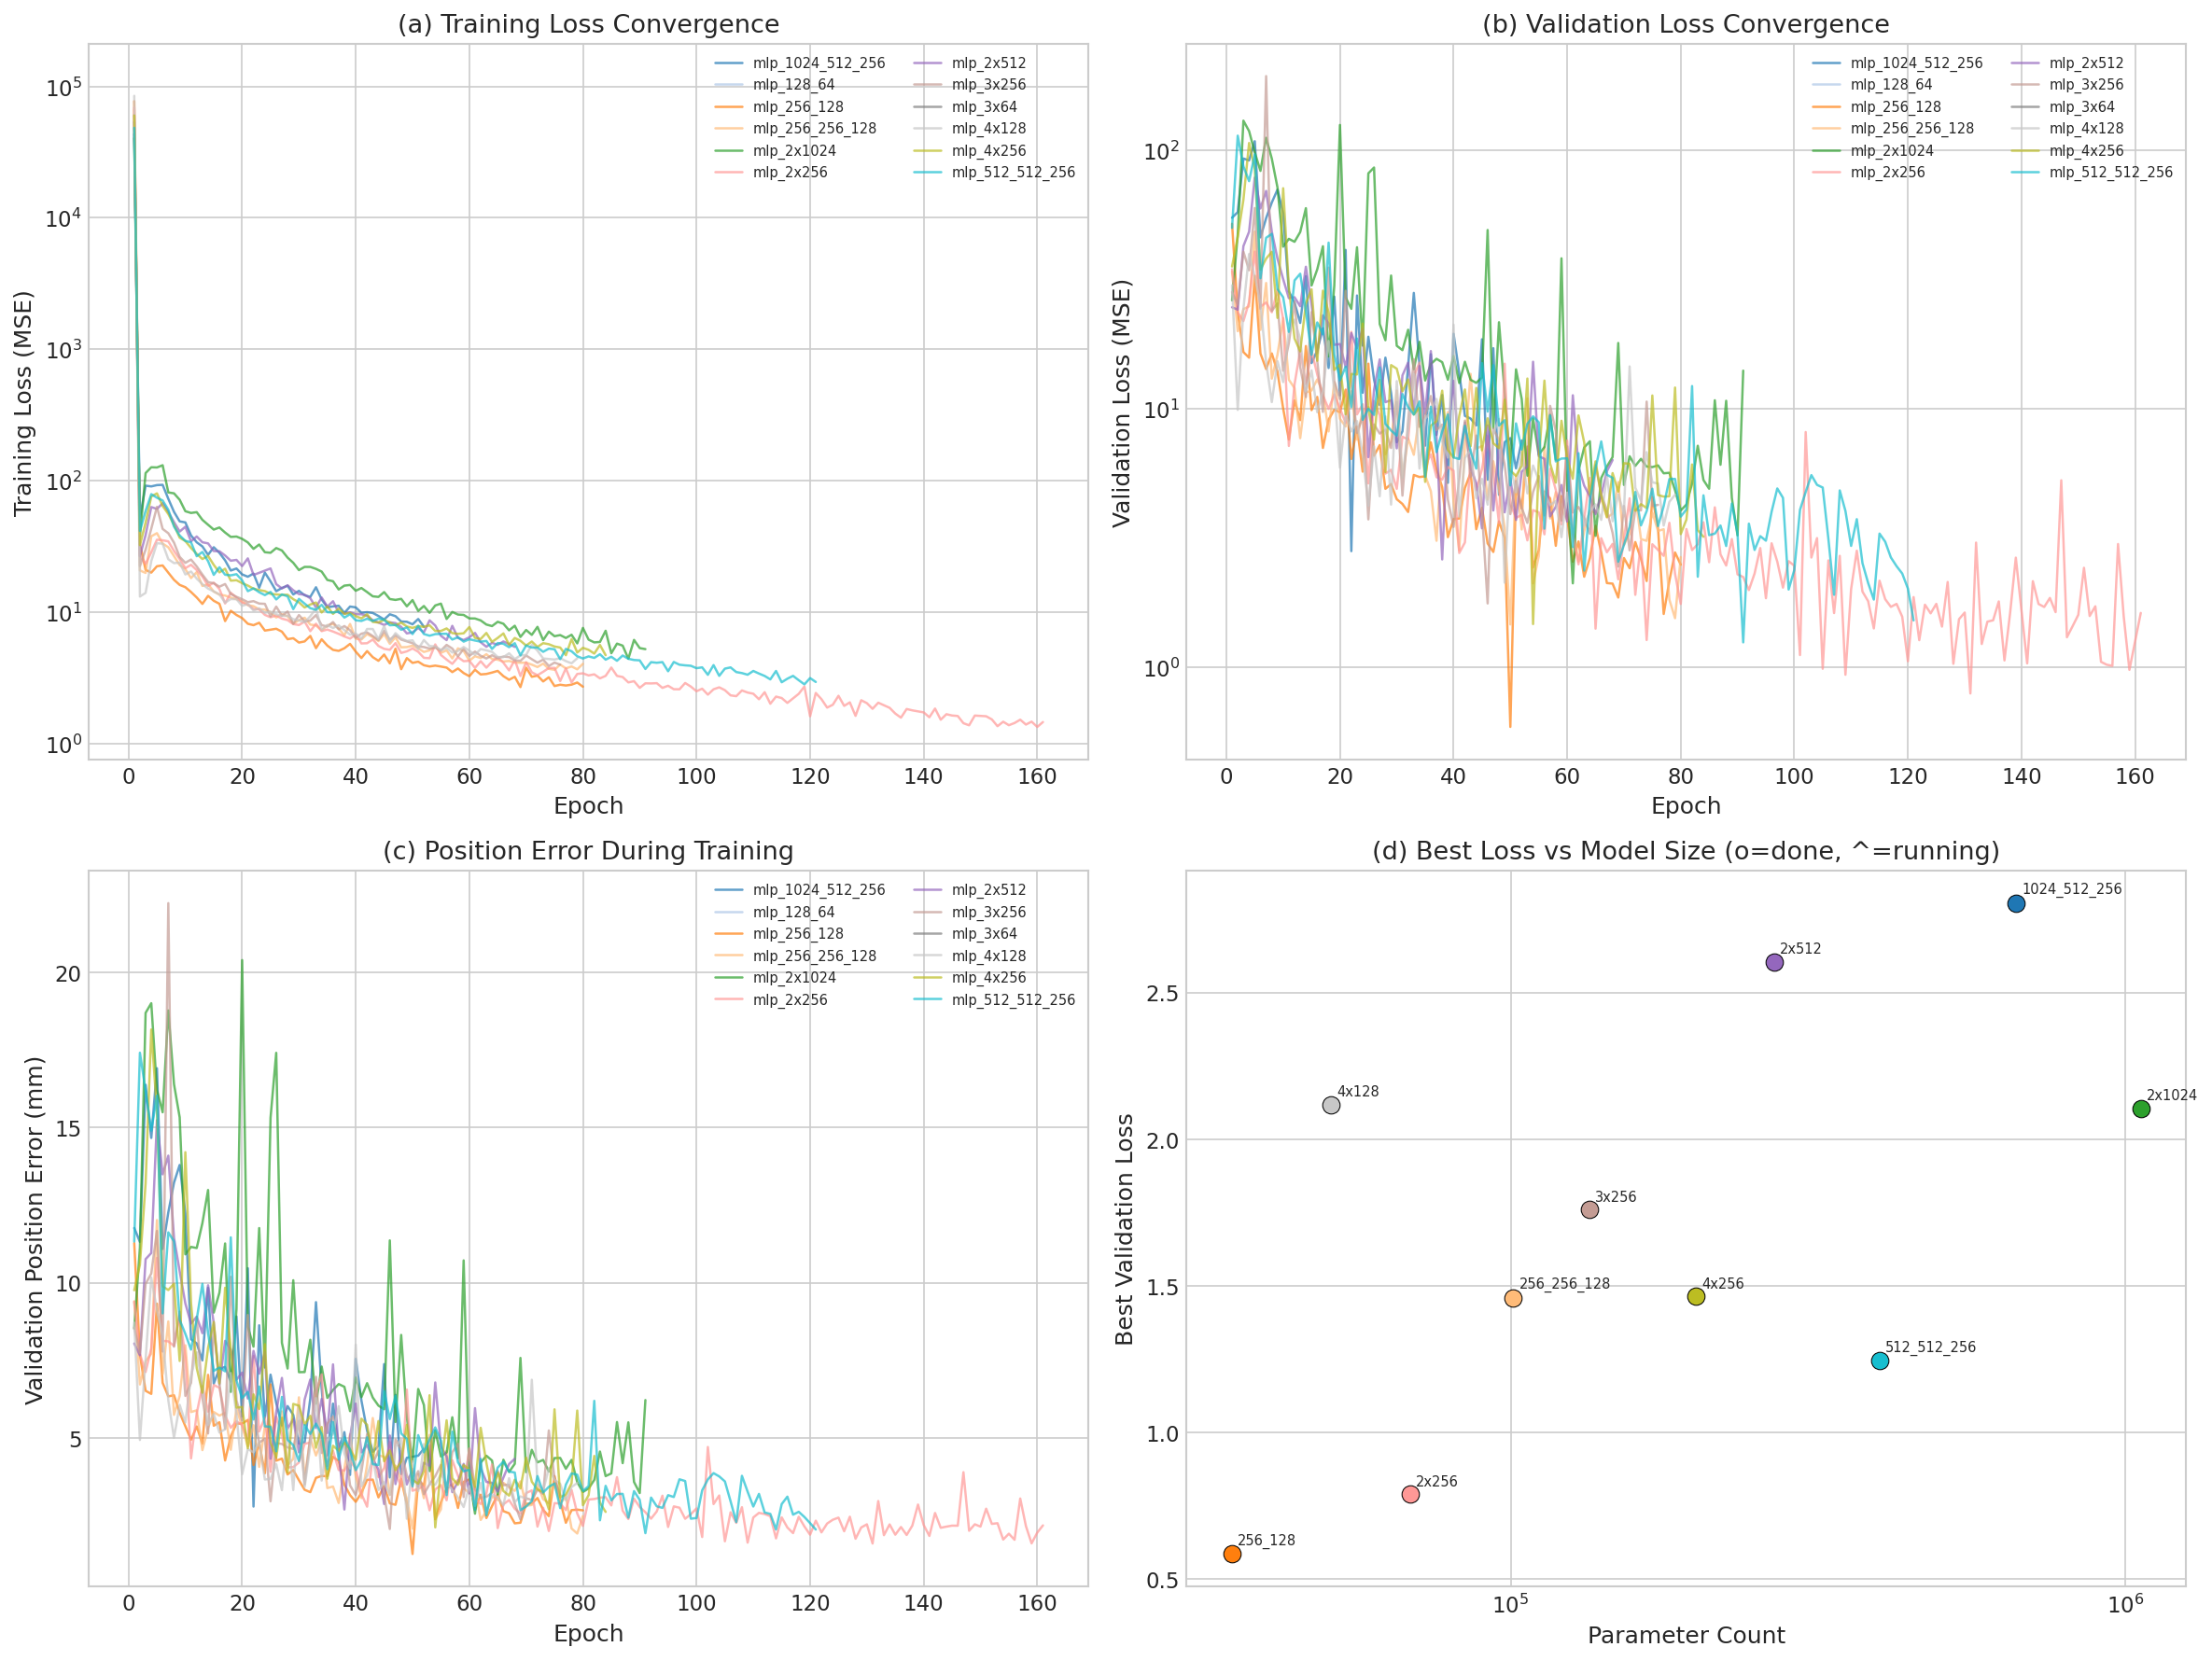
\includegraphics[width=0.82\linewidth]{../../experiments/gen_1/V1/analysis/convergence_analysis.png}
\caption{Training and validation loss trajectories for the 17 sweep runs.
  Small networks (bottom rows) converge within 50--100 epochs and then
  flatten under early stopping; the largest networks (top rows) are
  still improving when the 500-epoch cap triggers, consistent with the
  fixed-budget under-training hypothesis.}
\label{gen1:fig:convergence}
\end{figure}

Figure~\ref{gen1:fig:convergence} confirms the reading of
Table~\ref{gen1:tab:sweep}: convergence is clean for the small
architectures and evidently incomplete for the large ones within the
5M-sample budget.

\subsection{Error versus physics}

Figure~\ref{gen1:fig:err_mom} (left) shows the test-set position error
as a function of particle momentum $p$, and Figure~\ref{gen1:fig:err_mom}
(right) decomposes the residual into $x$-only and $y$-only components
for a representative model.

\begin{figure}[h]
\centering
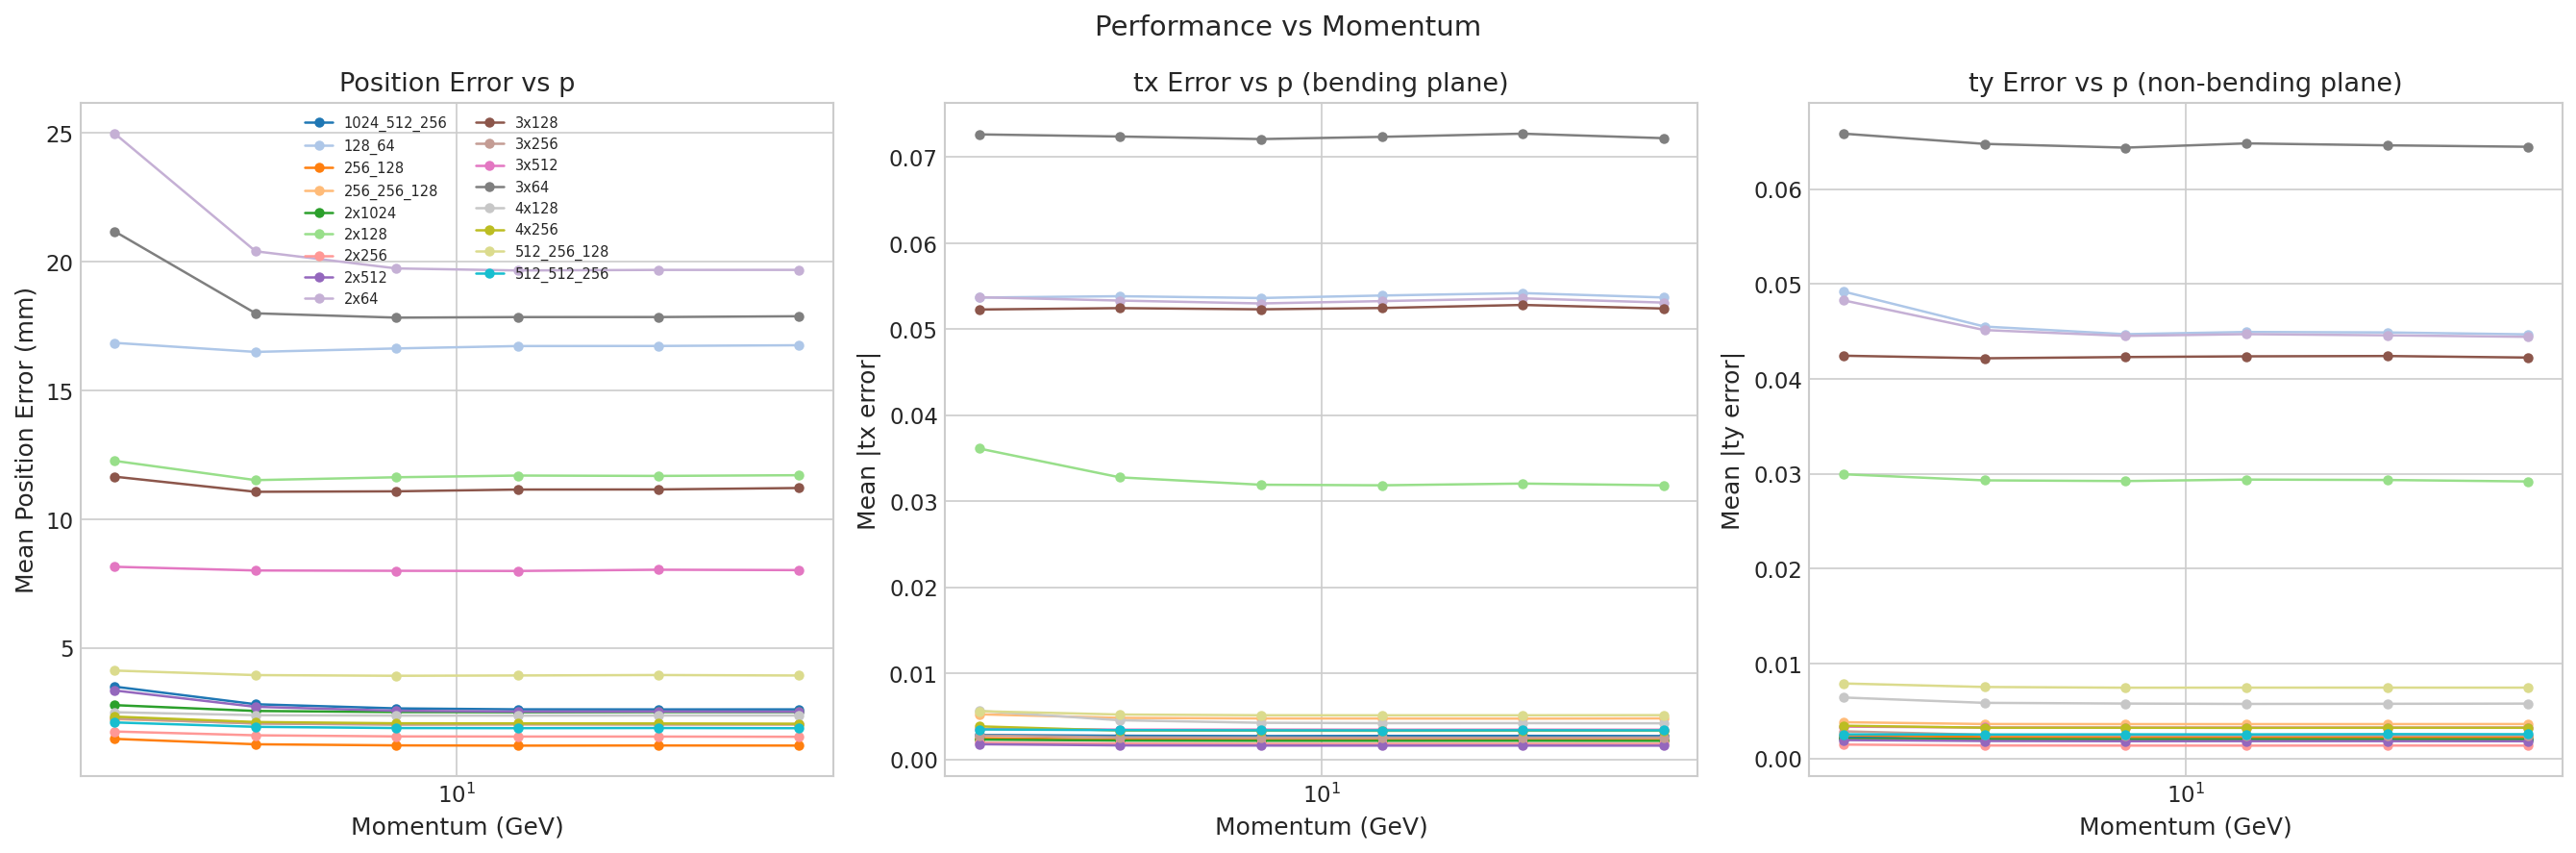
\includegraphics[width=0.47\linewidth]{../../experiments/gen_1/V1/analysis/error_vs_momentum.png}\hfill
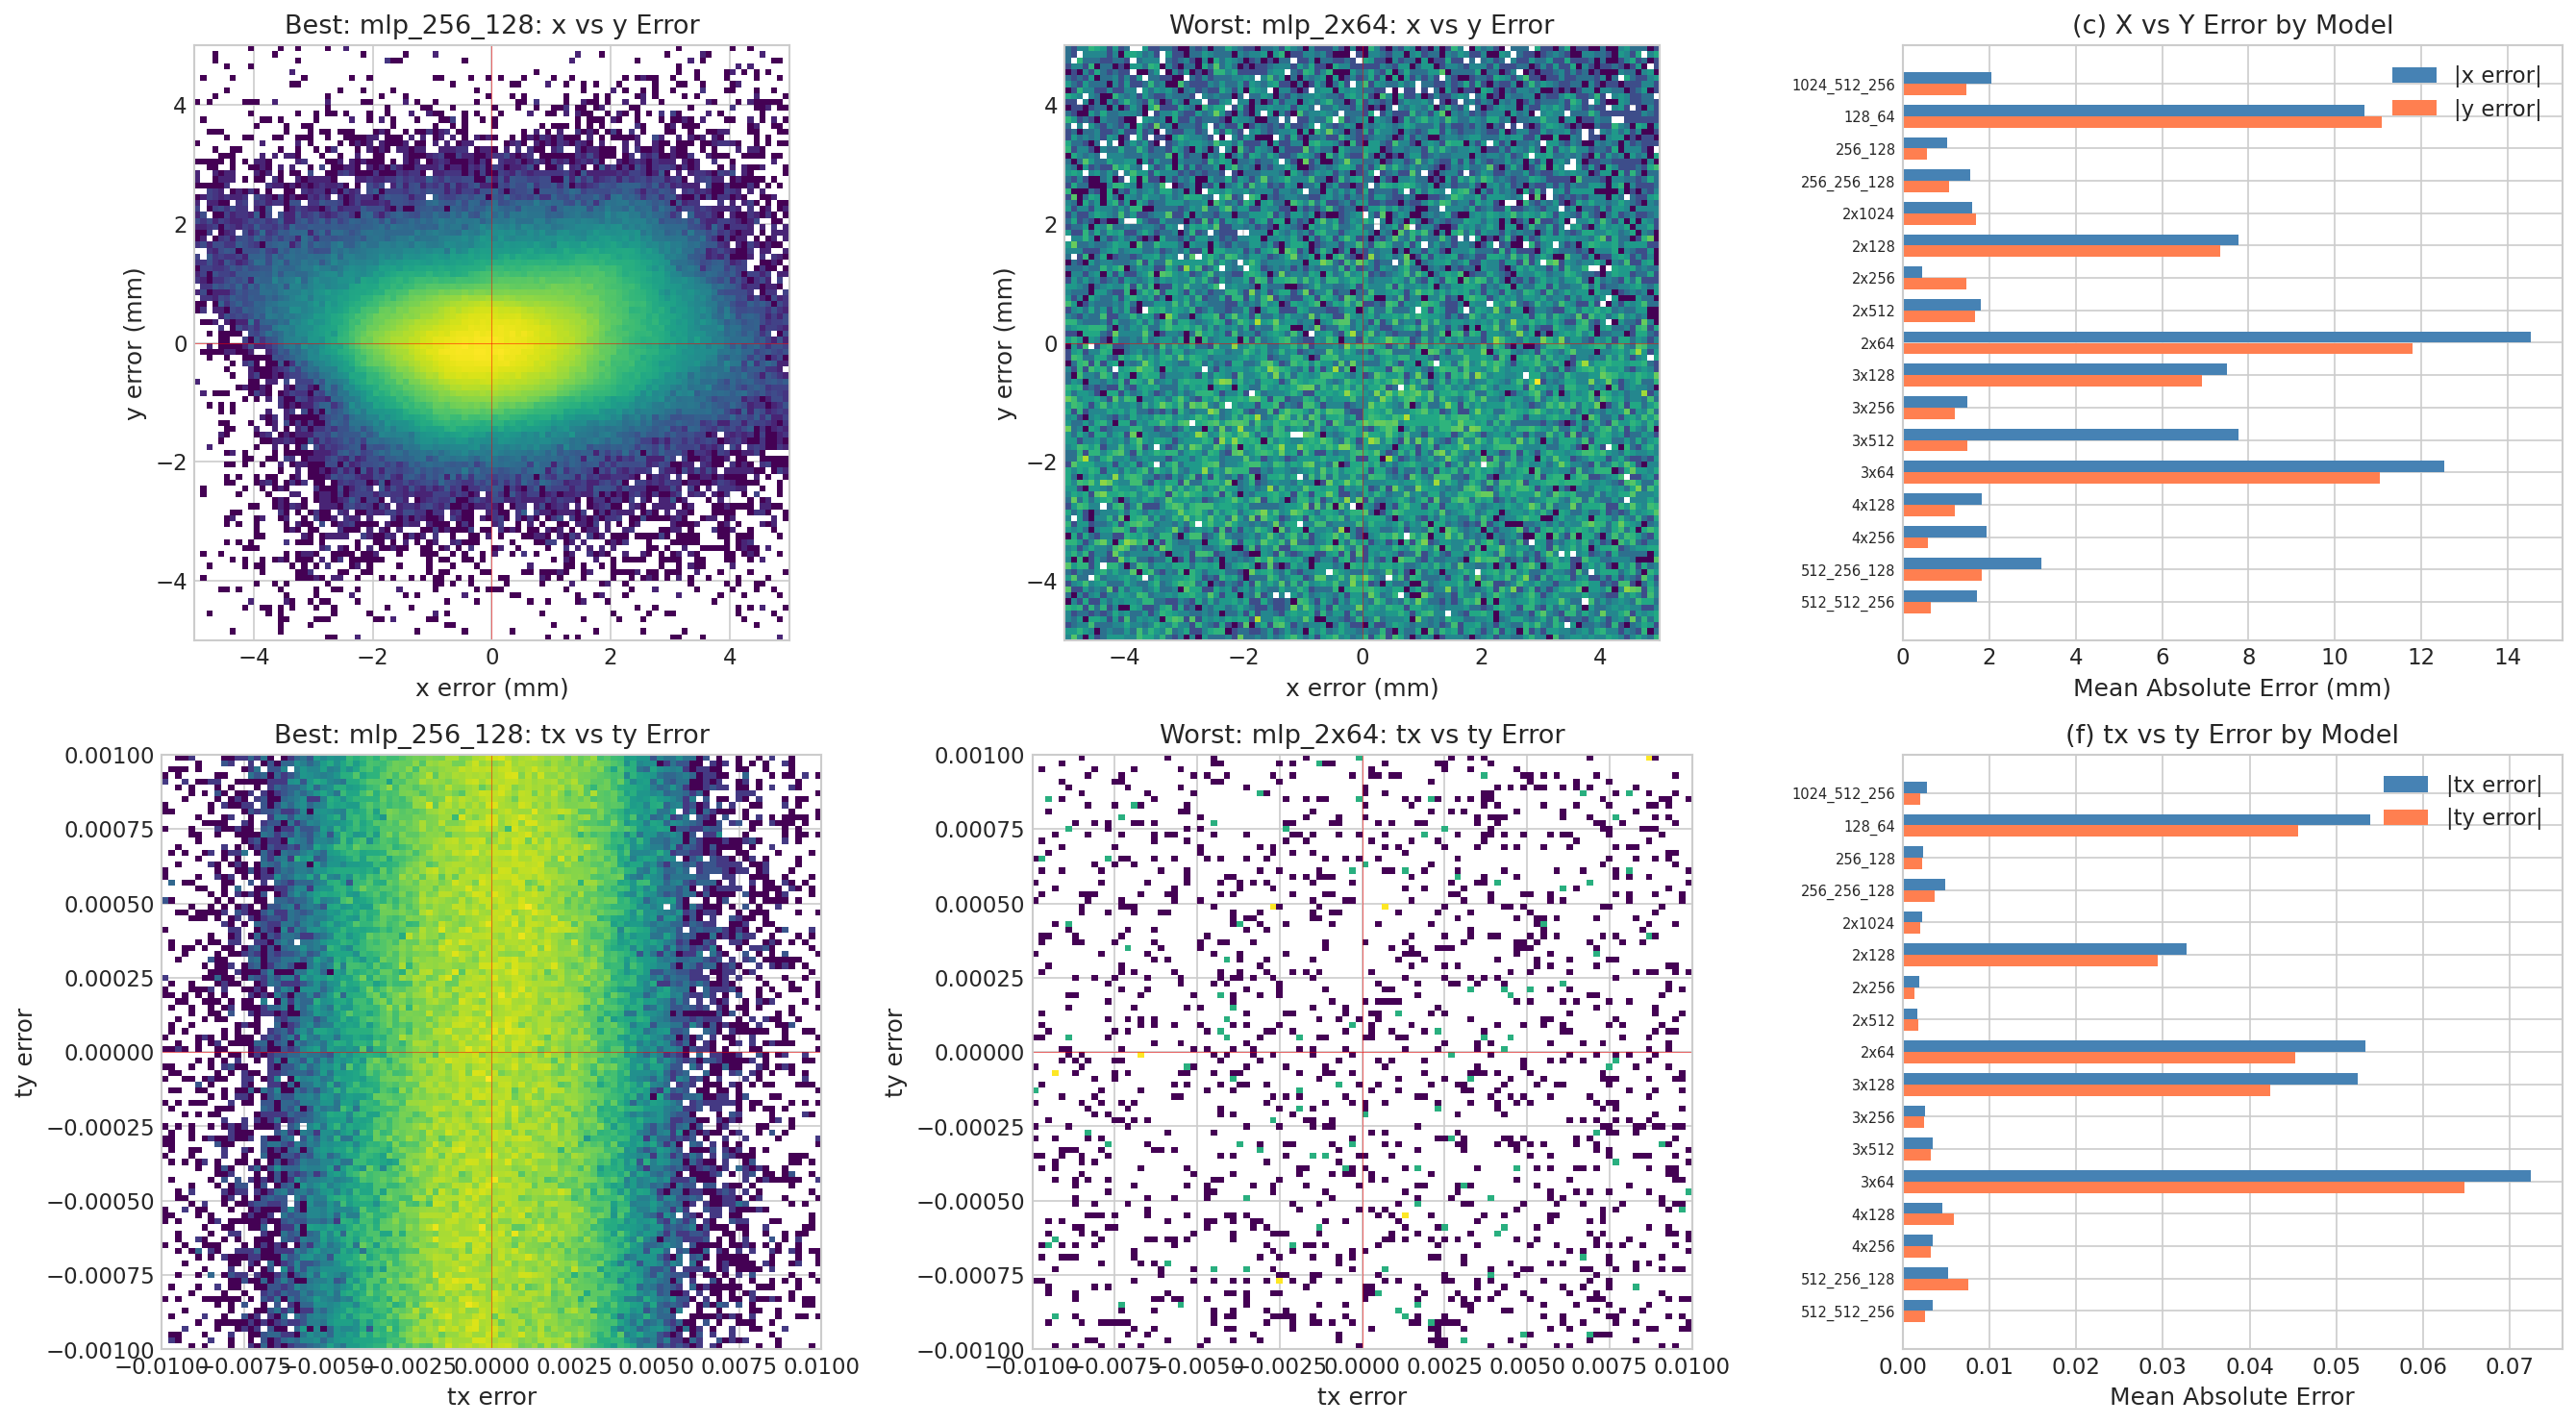
\includegraphics[width=0.47\linewidth]{../../experiments/gen_1/V1/analysis/xy_deflection_asymmetry.png}
\caption{Left: mean $\rho$ as a function of $p$. Low-momentum tracks
  ($p\lesssim\SI{5}{\giga\eV}/c$) incur larger residuals because the
  $\qop$-scaled bending in Eqs.~\eqref{gen1:eq:ode_tx}--\eqref{gen1:eq:ode_ty}
  is correspondingly larger, and small relative mis-estimates of the
  effective kick translate into proportionally larger absolute
  residuals.
  Right: $x$-only vs $y$-only residual distributions. The $x$
  component is systematically broader, consistent with the observation
  in Section~\ref{gen1:sec:physics} that the dominant field component
  $B_y$ kicks $t_x$ through Eq.~\eqref{gen1:eq:ode_tx}, while $t_y$ is
  only weakly coupled via the subdominant $B_x$, $B_z$ terms; after
  integration over $\dz$, the $x$-residual therefore accumulates more
  than the $y$-residual.}
\label{gen1:fig:err_mom}
\end{figure}

The $x/y$ asymmetry is not merely a curiosity: it is a direct
physics signature of the LHCb dipole geometry and provides a sanity
check on the training. A network that happened to produce symmetric
$x$/$y$ residuals would have learned a field that does not match the
real detector.

\subsection{Slope errors and Kalman implications}

The slope accuracy $\overline{\sigma_s}\sim 4\!\times\!10^{-3}$~rad
achieved across the competitive architectures translates, via
$t_x,t_y$, into a momentum-resolution-equivalent $\Delta p/p$ that is
several times larger than the existing RK4 extrapolator on the same
inputs. For ingestion by the downstream Kalman filter, which weights
each hit by the extrapolated covariance, a slope error at this level
would inflate the track-fit $\chi^2$ and degrade the ghost rejection
downstream. Closing this gap without blowing the parameter budget is
the central goal of the \texttt{gen\_2} work.

% -----------------------------------------------------------------------------
\section{Throughput and deployment}\label{gen1:sec:deployment}

\subsection{Benchmarks}

Figures~\ref{gen1:fig:throughput} and~\ref{gen1:fig:scatter_time}
report the inference throughput measurements for the sweep
architectures (test-time only, excluding data transfer).  The smallest
constant-memory-deployable networks reach sub-microsecond per-track
latencies on V100 and L40S, placing them within striking distance of
the existing RK4 kernel that they would replace.

\begin{figure}[h]
\centering
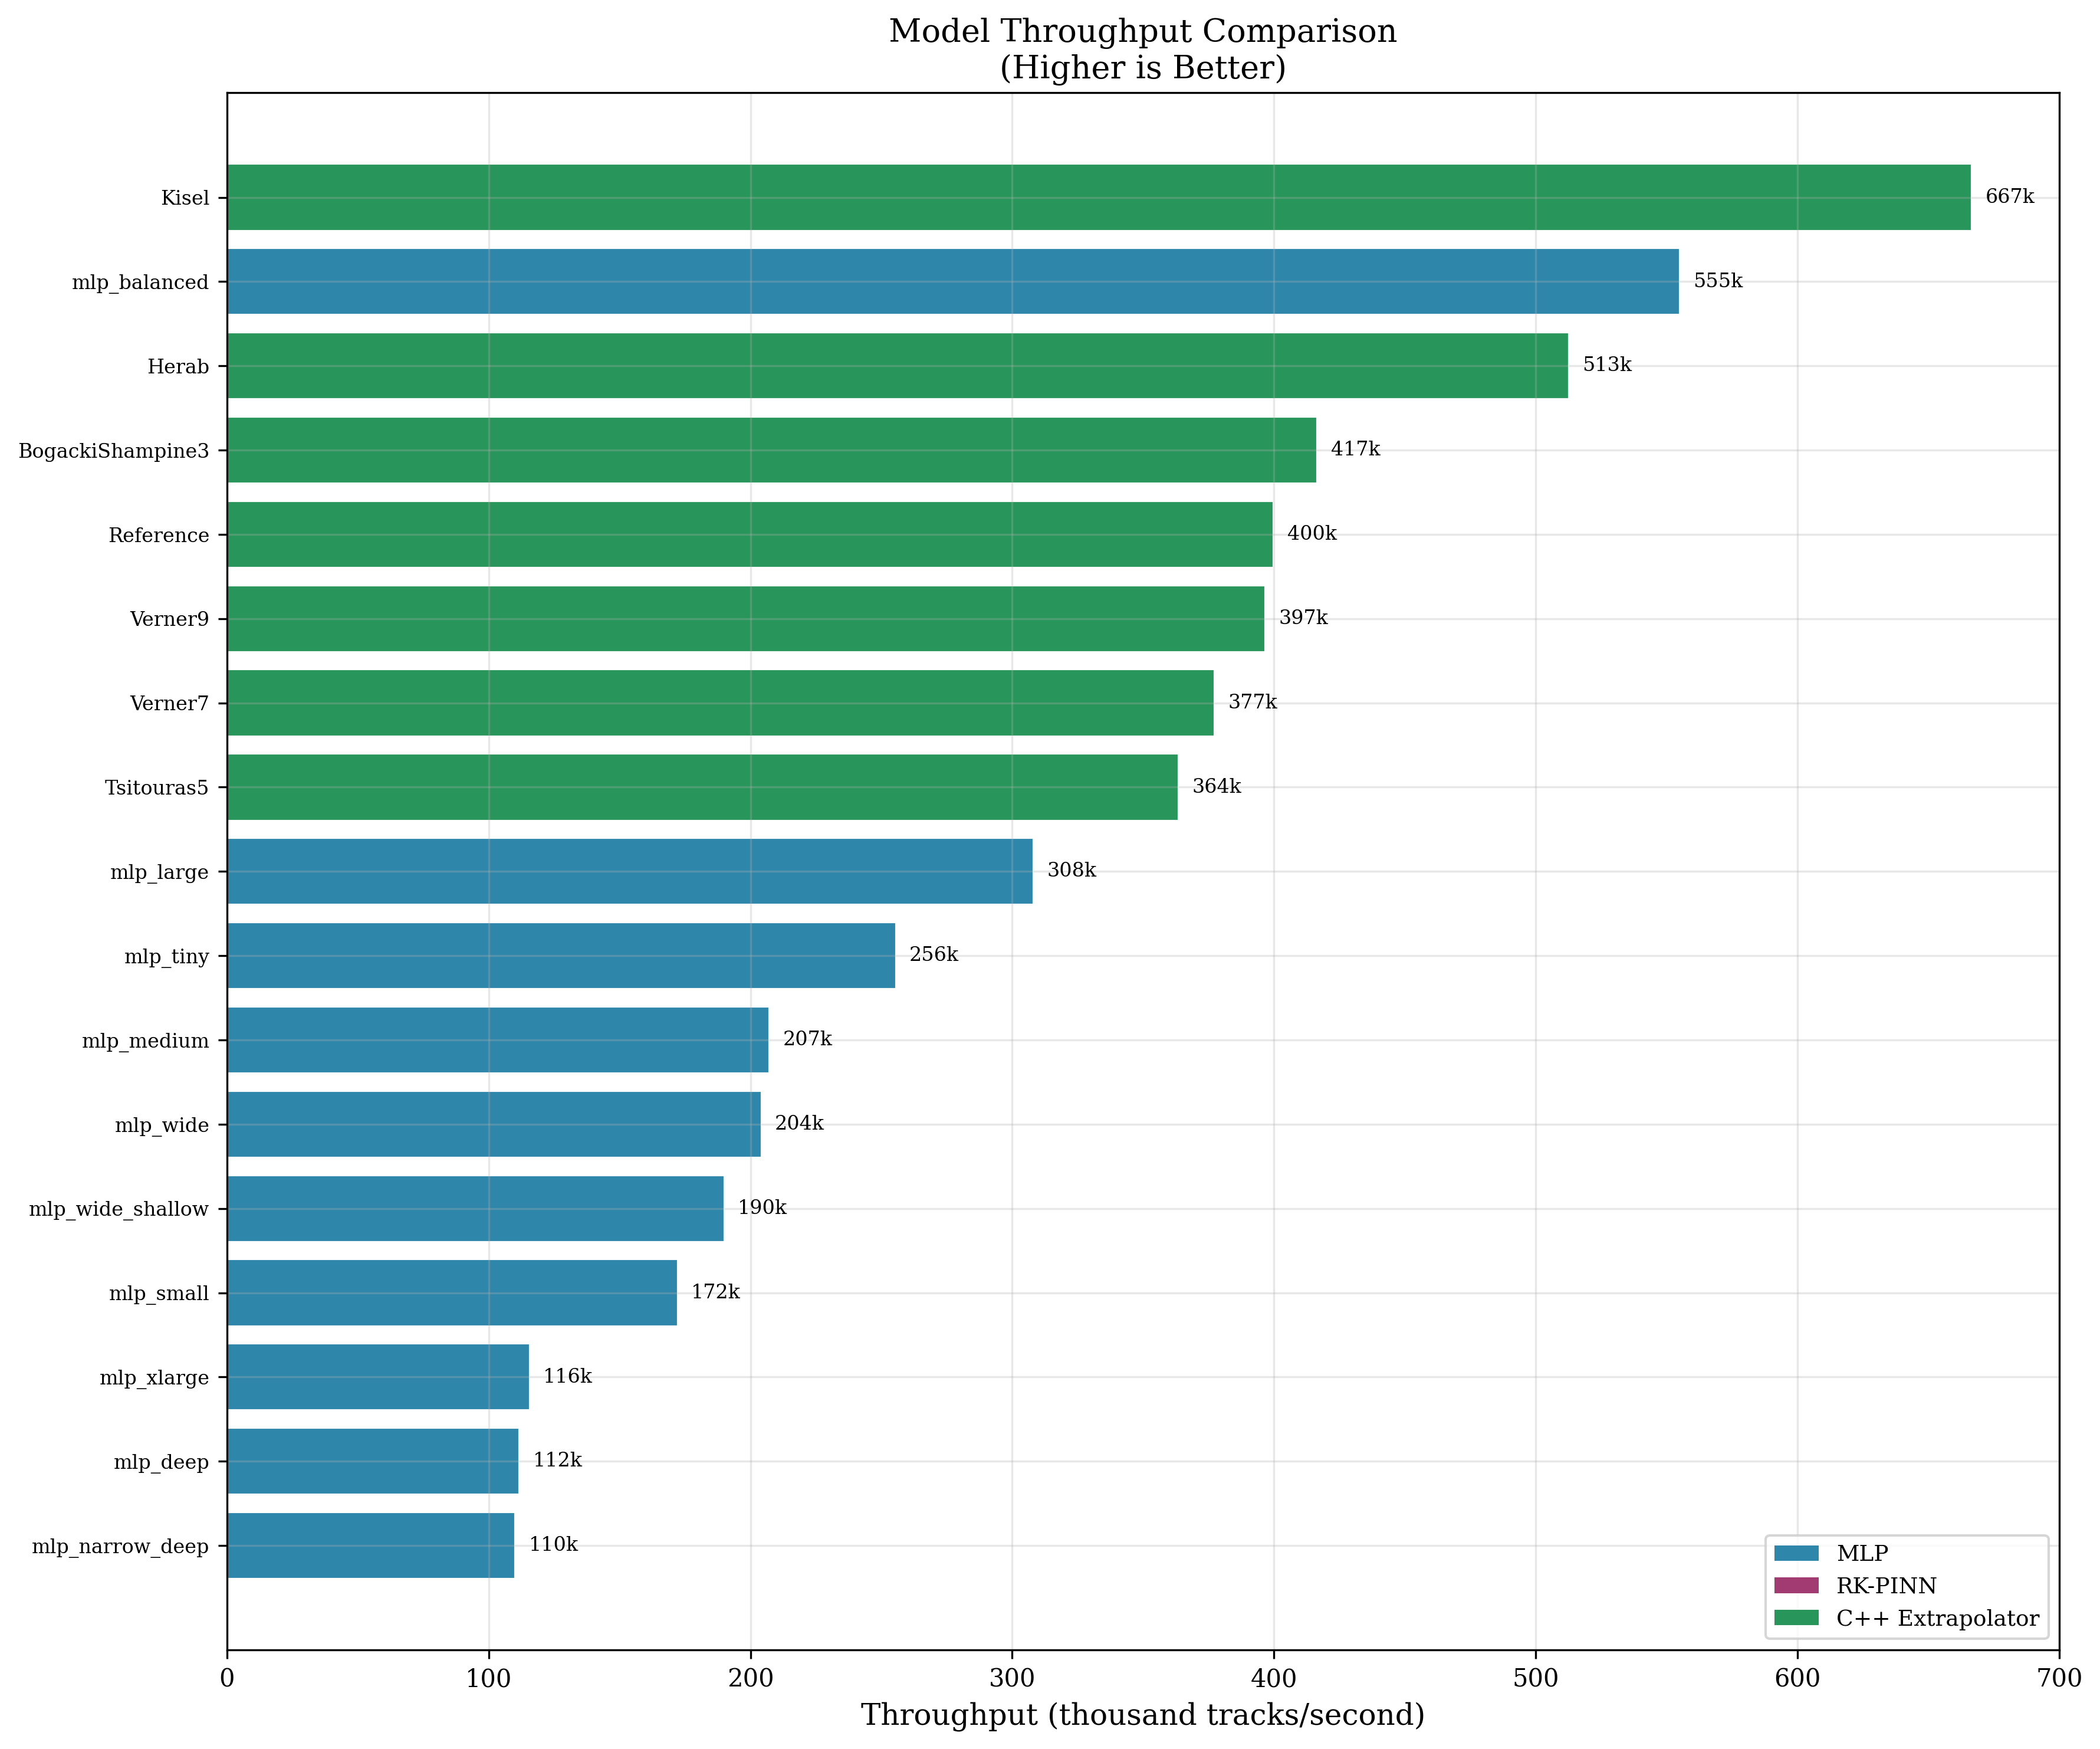
\includegraphics[width=0.78\linewidth]{../../experiments/gen_1/archive/paper_v1/throughput_comparison.png}
\caption{Inference throughput comparison across the 17 sweep
  architectures. The small deployable networks (left) achieve
  throughputs within an order of magnitude of the RK4 baseline.}
\label{gen1:fig:throughput}
\end{figure}

\begin{figure}[h]
\centering
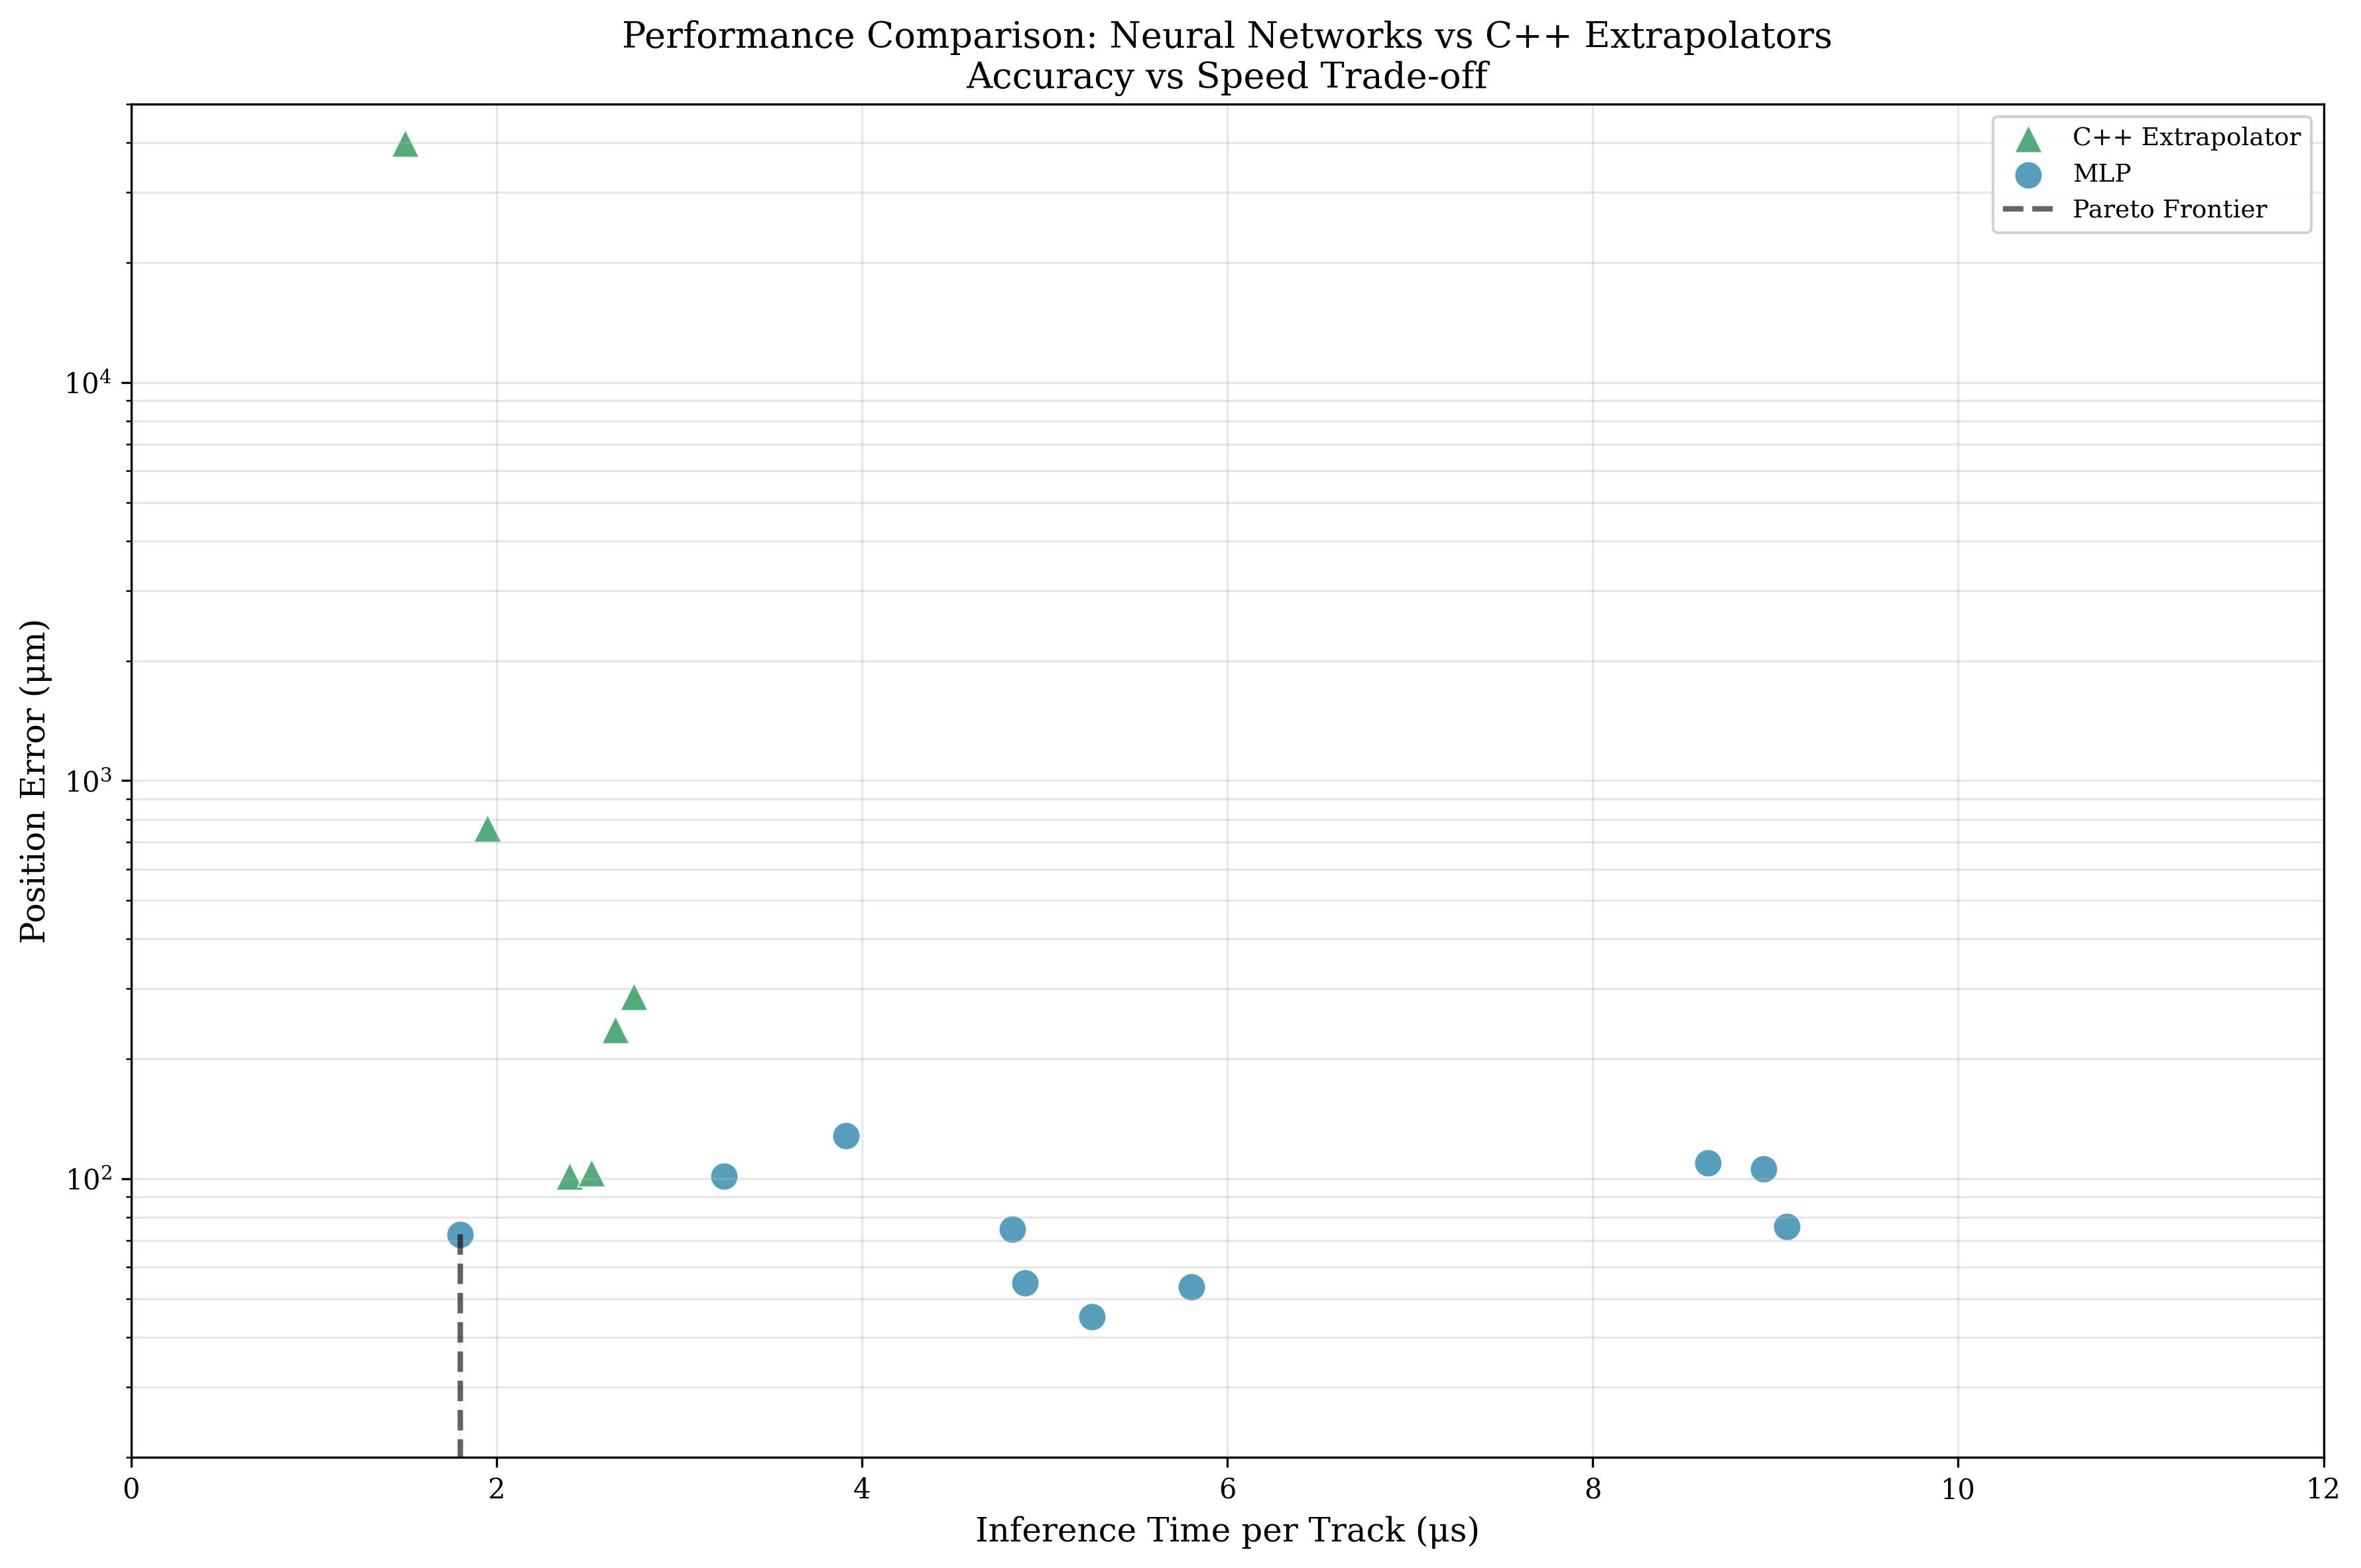
\includegraphics[width=0.78\linewidth]{../../experiments/gen_1/archive/paper_v1/scatter_all_models_accuracy_vs_time.png}
\caption{Accuracy vs wall-time for the full sweep. The
  \SI{64}{\kilo\byte}-deployable region is the lower-left corner. The
  set of Pareto-optimal deployable points defines the achievable
  accuracy/latency envelope for a purely data-driven MLP in the Allen
  HLT1 chain under the current sampling strategy.}
\label{gen1:fig:scatter_time}
\end{figure}

\subsection{C++ integration path}

The deployment path from PyTorch to Allen is:
\begin{enumerate}\setlength{\itemsep}{1pt}
\item \texttt{export\_to\_c\_binary.py} exports the trained weights (and
  the z-score normalisation constants) as a flat little-endian binary
  blob next to the checkpoint;
\item \texttt{TrackMLPExtrapolator.cpp} (571 lines, Eigen-based)
  consumes that blob, implements the forward pass in dense matrix form,
  and exposes a C ABI suitable for wrapping into the Allen algorithm
  registry;
\item an identical reference implementation in pure NumPy is kept
  alongside for cross-validation against the PyTorch evaluation loop.
\end{enumerate}
No deployment is performed in this report --- the C++ path has been
validated on CPU only, and the final integration into the Allen GPU
pipeline is deferred to a later phase conditional on an MLP meeting
both the accuracy and the \SI{64}{\kilo\byte} constraint
simultaneously.

% -----------------------------------------------------------------------------
\section{Limitations and transition}\label{gen1:sec:limitations}

Four limitations of the \texttt{gen\_1} sweep explicitly motivate the
\texttt{gen\_2} work:

\begin{itemize}\setlength{\itemsep}{2pt}
\item[(a)] \textbf{Fixed-budget under-training.} Every sweep run uses
  \texttt{max\_samples}$=\num{5e6}$, i.e.\ 10\% of the on-disk dataset.
  The largest networks clearly have not converged at this budget
  (Figure~\ref{gen1:fig:convergence}), so the measured
  accuracy/capacity scaling is biased in favour of the small networks
  and against the large ones. This must be corrected before drawing any
  general conclusion about MLP scaling for this task.
\item[(b)] \textbf{Best accuracy is not deployable.} The
  mid-to-large architectures that sit on or near the Pareto front all
  violate the \SI{64}{\kilo\byte} budget.  The deployable subset
  (\texttt{2x64}, \texttt{3x64}, \texttt{128\_64}) achieves
  $\overline{\rho}\gtrsim\SI{1}{\mm}$, which is at the edge of what the
  Kalman filter tolerates at the VELO exit.
\item[(c)] \textbf{No physics regularisation.} The network is trained
  purely by output-space MSE and has no gradient-level awareness of
  Eqs.~\eqref{gen1:eq:ode_x}--\eqref{gen1:eq:ode_ty}. In particular,
  there is no enforcement of momentum conservation, no penalty against
  predictions that violate the energy surface $\|\hat{t}\|^2 \leq
  \|t\|_{\max}^2$, and no RK4-consistency term.
\item[(d)] \textbf{Slope accuracy too loose for Kalman.} As
  discussed in Section~\ref{gen1:sec:analysis}, the plateau
  $\overline{\sigma_s}\sim 4\!\times\!10^{-3}$~rad is insufficient for
  tight downstream track fitting.
\end{itemize}

The follow-on companion work is split in two:
\begin{itemize}\setlength{\itemsep}{2pt}
\item \texttt{gen2\_old\_data\_results.tex} retrains on the same
  dataset with physics-informed baselines --- a PINN with an ODE
  residual loss of the form in Eqs.~\eqref{gen1:eq:ode_x}--\eqref{gen1:eq:ode_ty}
  following~\cite{Raissi2019,Wang2021,Krishnapriyan2021}, and an
  RK\_PINN that explicitly embeds the four-stage Butcher tableau into the
  forward pass. This targets limitations (c) and (d).
\item \texttt{gen2\_new\_data\_results.tex} extends the training set
  to cover the LHCb VELO inter-sensor spacing regime $\dz\in[25,
  30]$~\SI{}{\mm} and extends momentum up to $p=\SI{200}{\giga\eV}/c$,
  introduces the v2 fixes (PINN\_v2, NeuralRK4) motivated by
  neural-ODE style residuals~\cite{Chen2018}, and trains on the full
  dataset to eliminate the fixed-budget confound. This targets
  limitations (a) and (b).
\end{itemize}

% -----------------------------------------------------------------------------
\section{Reproducibility}\label{gen1:sec:reproducibility}

All results in this report are reproduced from:
\begin{itemize}\setlength{\itemsep}{1pt}
\item Environment: \texttt{conda activate TE} (Python 3.10, PyTorch
  2.9.1+cu128); see \texttt{TrackExtrapolation/environment.yml} for the
  full pinning;
\item Random seed: 42 (applied to NumPy, PyTorch, and the CUDA RNG);
\item MLflow experiment: \texttt{V1\_MLP\_sweep} under the default
  local tracking URI;
\item Sweep JSON: \texttt{experiments/gen\_1/V1/analysis/v1\_sweep\_results.json};
\item Data generation: \texttt{experiments/gen\_1/V1/data\_generation/\{generate\_data.py,\ rk4\_propagator.py\}};
\item Analysis notebook:
  \texttt{experiments/gen\_1/V1/analysis/v1\_model\_characterisation.ipynb};
\item C++ reference:
  \texttt{TrackExtrapolation/src/TrackMLPExtrapolator.cpp} (Eigen,
  571 lines); export pipeline
  \texttt{experiments/gen\_1/V1/analysis/export\_to\_c\_binary.py}.
\end{itemize}
Per the caveat in Section~\ref{gen1:sec:data}, exact re-run of the sweep on
the \emph{current} \texttt{train\_50M.npz} will not reproduce the
numbers in Table~\ref{gen1:tab:sweep} at the quoted precision; to
reproduce, the fixed-$\dz$ data generator must be restored from git
history first.

% -----------------------------------------------------------------------------
\begin{thebibliography}{99}
\small

\bibitem{LHCbDetector2008}
LHCb Collaboration, ``The LHCb Detector at the LHC,''
\emph{JINST} \textbf{3}, S08005 (2008). DOI:
\href{https://doi.org/10.1088/1748-0221/3/08/S08005}{10.1088/1748-0221/3/08/S08005}.

\bibitem{Allen2020}
R.~Aaij \emph{et al.}, ``Allen: A high-level trigger on GPUs for LHCb,''
\emph{Comput. Softw. Big Sci.} \textbf{4}, 7 (2020).
\href{https://doi.org/10.1007/s41781-020-00039-7}{doi:10.1007/s41781-020-00039-7}.

\bibitem{Fruhwirth1987}
R.~Fr{\"u}hwirth, ``Application of Kalman filtering to track and vertex
fitting,'' \emph{Nucl. Instrum. Meth. A} \textbf{262}, 444--450 (1987).

\bibitem{Elfwing2018}
S.~Elfwing, E.~Uchibe, K.~Doya, ``Sigmoid-weighted linear units for
neural network function approximation in reinforcement learning,''
\emph{Neural Networks} \textbf{107}, 3--11 (2018).
arXiv:\href{https://arxiv.org/abs/1702.03118}{1702.03118}.

\bibitem{GlorotBengio2010}
X.~Glorot, Y.~Bengio, ``Understanding the difficulty of training deep
feedforward neural networks,'' \emph{AISTATS} (2010).

\bibitem{LoshchilovHutter2019}
I.~Loshchilov, F.~Hutter, ``Decoupled weight decay regularization,''
\emph{ICLR} (2019).
arXiv:\href{https://arxiv.org/abs/1711.05101}{1711.05101}.

\bibitem{KingmaBa2015}
D.~P.~Kingma, J.~Ba, ``Adam: A method for stochastic optimization,''
\emph{ICLR} (2015).
arXiv:\href{https://arxiv.org/abs/1412.6980}{1412.6980}.

\bibitem{Raissi2019}
M.~Raissi, P.~Perdikaris, G.~E.~Karniadakis, ``Physics-informed neural
networks: A deep learning framework for solving forward and inverse
problems involving nonlinear partial differential equations,''
\emph{J. Comput. Phys.} \textbf{378}, 686--707 (2019).
\href{https://doi.org/10.1016/j.jcp.2018.10.045}{doi:10.1016/j.jcp.2018.10.045}.

\bibitem{Wang2021}
S.~Wang, Y.~Teng, P.~Perdikaris, ``Understanding and mitigating gradient
flow pathologies in physics-informed neural networks,''
\emph{SIAM J. Sci. Comput.} \textbf{43}, A3055--A3081 (2021).
\href{https://doi.org/10.1137/20M1318043}{doi:10.1137/20M1318043}.

\bibitem{Krishnapriyan2021}
A.~S.~Krishnapriyan, A.~Gholami, S.~Zhe, R.~Kirby, M.~W.~Mahoney,
``Characterizing possible failure modes in physics-informed neural
networks,'' \emph{NeurIPS} (2021).
arXiv:\href{https://arxiv.org/abs/2109.01050}{2109.01050}.

\bibitem{Chen2018}
R.~T.~Q.~Chen, Y.~Rubanova, J.~Bettencourt, D.~Duvenaud, ``Neural
ordinary differential equations,'' \emph{NeurIPS} (2018).
arXiv:\href{https://arxiv.org/abs/1806.07366}{1806.07366}.

\end{thebibliography}

% =============================================================================
% Outstanding TODOs / notes for reviewer
% =============================================================================
% TODO: The request brief suggested "best pos ~0.2 mm" in the executive
%       summary. The JSON v1_sweep_results.json yields best pos_mean =
%       1.017 mm (mlp_3x64). The report uses the verified JSON number,
%       not the brief's 0.2 mm value. Please confirm this is the intended
%       figure or point me to the source of the 0.2 mm claim.
% TODO: The 64 kB deployability column counts parameters only; once the
%       normalisation constants (means + stds, 20 float32 values) are
%       added the budget tightens by 80 bytes, still well within margin.
%       Activation buffers and kernel stack are on-chip and not counted
%       against constant memory.
% TODO: Compilation of this file with pdflatex has NOT been attempted in
%       the current environment (no shell execution available to the
%       report writer). Please run:
%           cd docs/reports && pdflatex -interaction=nonstopmode gen1_results.tex
%           cd docs/reports && pdflatex -interaction=nonstopmode gen1_results.tex
%       and confirm that figure paths resolve and the bibliography renders.
% =============================================================================

\end{document}
